\chapter{A Description of DAMOCLES}\label{chp:chp2}

%\begin{flushright}
%  {\em QUOTE GOES HERE }\\
%
%\ \
%
%\normalsize
%{AUTHOR}  
%\end{flushright}


\section{Monte Carlo Methods}

\noindent{The name ``Monte Carlo" describes a class of modelling techniques that employ a stochastic approach to simulating mathematical and physical situations that are otherwise difficult or impossible to solve.  By repeatedly sampling random numbers from a probability distribution, numerical results to non-analytic problems may be obtained.  The approach was first used by researchers at Los Alamos in the late 1940s who adopted the method to model the transport of neutrons \citep{Metropolis1949}.  It is from the code name for this project, ``Monte Carlo", that the methods derive their name.}

As the available computing power increased over the following decades, Monte Carlo methods became more and more useful as a means of solving complex problems and are now used widely across numerous fields including mathematics, statistics, engineering, finance, the physical sciences and many others.  The nature of the approach means that they are particularly well-suited to problems with multiple degrees of freedom, and especially when any of these degrees are coupled.  By using random numbers to represent quantities that parametrise a physical problem, a solution to the problem may be sought using a pseudo-random number generator.   It must be the case that the quantities that characterise the problem may be represented by a continuous distribution in the range [0,1] in order that the randomly generated numbers may be translated into physical properties \citep{Shreider1966}.  

Having thus obtained a random set of physical parameters, a model is constructed and an output - a ``possible outcome" - is obtained.  By repeatedly iterating this process with new randomly-generated inputs each time, many possible outcomes are produced and a probability distribution is built up.  The interpretation of the outputted probability distribution is dependent on the manner of utilisation of the Monte Carlo method.  For example, the procedure may be used to find the mean-free paths of millions of energy packets where the resulting probability distribution of the final frequencies of the packets is equivalent to an energy distribution.  This is the process that I make use of and I will discuss it in more detail throughout this chapter.

More recently Monte Carlo methods have been applied to Bayesian statistical analyses that seek to uncover a complete multidimensional probability distribution describing the parameter space of a particular model.  The intention is to derive not just a well-fitting model but to understand how variations in a given parameter affect the likelihood that the model is representative of the data.  These investigations of parameter space generally adopt a Markov Chain Monte Carlo (MCMC) approach.  Where a Monte Carlo method generates a sample from a required distribution, a MCMC technique draws samples according to a predefined set of rules that result in a sequence of samples called a Markov Chain.  These methods allow for a more intelligent and efficient sampling of parameter space \citep{Metropolis1953, Hastings1970, Gilks1996}.  

Clearly, Monte Carlo simulations are limited by their finite nature and will never produce a perfect solution.  However, this does not mean that Monte Carlo simulations are lacking in rigour.  It may be shown that the error in a Monte Carlo model is approximately $\sim \frac{1}{\sqrt{n}}$ for large $n$, where $n$ is the number of quanta used in the simulation \citep{Press2007}.  The error may therefore be made as small as required by increasing the number of quanta used in the simulation subject to the restrictions of computing time and expense.

In the next section, I discuss the use of Monte Carlo methods as applied to radiative transfer problems and specifically to DAMOCLES.  I discuss the computational aspects of my work and the architecture of the code in section \ref{damocles_struct} before finally discussing the limitations of the code and its potential for future developments in section \ref{limitations}.

\section{Radiative Transfer and the Monte Carlo Method}
\label{rt}

The application of Monte Carlo codes to radiative transfer problems in astrophysics has a strong history.  Numerous codes that utilise this stochastic methodology have been written in the past few decades in order to model the transport of energy packets through various media, for example Mocassin, TORUS, Hyperion, SKIRT, LIME, RATRAN, Cloudy and many others \citep{Harries2000, Hogerheijde2000, Baes2003, Ercolano2003, Ercolano2005, Brinch2010, Robitaille2011, Ferland2013}.  The energy to be transported throughout the region of interest is discretised into packets and the path of each packet is calculated according to the properties of the environments that it passes through during its lifetime.  Collating the escaped packets at the end of the simulation produces an energy distribution that may be compared to observed photometric or spectral data. 

In addition to numerous codes that treat the continuous emission and absorption of energy in dusty environments in order to produce and fit spectral energy distributions (SEDs), there also exist several Monte Carlo radiative transfer codes that model the transfer and interaction of line emission through a 3D nebula in order to produce a synthetic spectrum (e.g. Brute \citep{Thomas2003} and ARTIS \citep{Kromer2009}).  These latter models frequently employ an approximation known as the Sobolev approximation \citep{Sobolev1957}.  This method allows spectral lines in media moving with high velocity gradients to be treated more simply by solving the radiative transfer equation locally under the assumption that the macroscopic velocity gradient is more important than the thermal line width.  Models of supernovae have been produced using both approaches and well-fitting spectra and SEDs have been generated but never, according to the best of my knowledge, has the Monte Carlo methodology been employed to produce sophisticated models of individual line profiles in expanding dusty regions.  In this new code, DAMOCLES, we seek to apply the technique to an expanding dusty medium in order to consider the effects of dust on a single emitted line profile.  

Previous work by Leon Lucy has considered the problem of computing the spectra of supernovae using Monte Carlo techniques \citep{Lucy1987,Lucy1999,Lucy2002,Lucy2003,Lucy2005c,Lucy2005b}.  In particular Lucy and colleagues consider dust-induced asymmetric line profiles in the ejecta of CCSNe and they have published results derived both analytically and using simple Monte Carlo simulations \citep{Lucy1989,Lucy1991}.  These simulations appear to be the only published instances of a numerical approach to studying this spectral feature.  The DAMOCLES code adopts the same technique as the original modelling by Leon Lucy but allows for a considerably more complex treatment of the composition, geometry and motion of the dusty medium.

Radiative transfer methods as applied to supernovae generally treat a wide wavelength range and seek to conserve the total energy.  In the case of SED modelling, this is often achieved by dividing the total energy into packets of equal weight and energy, and iteratively determining the temperature and ionisation structure.  In this work, the approach we adopt is somewhat simpler as only a very narrow wavelength range need be considered.  Rather than seeking to conserve the total energy, we assume that any packet absorbed by dust would be re-emitted outside the wavelength range of interest and thus no longer contributes to the resulting line profile.  Any absorbed packet is therefore removed from circulation.  In addition to this, the absorption and scattering of radiation by dust is independent of temperature and there is therefore no need to calculate temperatures throughout the nebula.  Similarly, the use of the Sobolev approximation (described above) is unnecessary here as only a single line or doublet is ever treated and a comparatively narrow wavelength range considered. 

The subtleties of the problem we consider here lie in the treatment of an atmosphere expanding as fast as 10\% of the speed of light, and in the complexities of the dusty medium itself.  Lorentz transforms must be carefully applied in order that packets experience the appropriate degree of frequency shifting at emission and at each subsequent scattering event.  In this respect, the code is analogous to Monte Carlo radiative transfer models of electron scattering published by \citep{Auer1972,Hillier1991}.  Indeed, similar features are observed in the outputs of both.

Throughout this section, I will describe the principles, assumptions and techniques adopted in the production of DAMOCLES (see Figure \ref{fig:flowchart}) before I move on to address the mechanics and architecture of the code itself.  DAMOCLES stands for \textbf{D}ust-\textbf{A}ffected \textbf{M}odels \textbf{O}f \textbf{C}haracteristic \textbf{L}ine \textbf{E}mission in \textbf{S}upernovae.


\begin{figure}
\centering
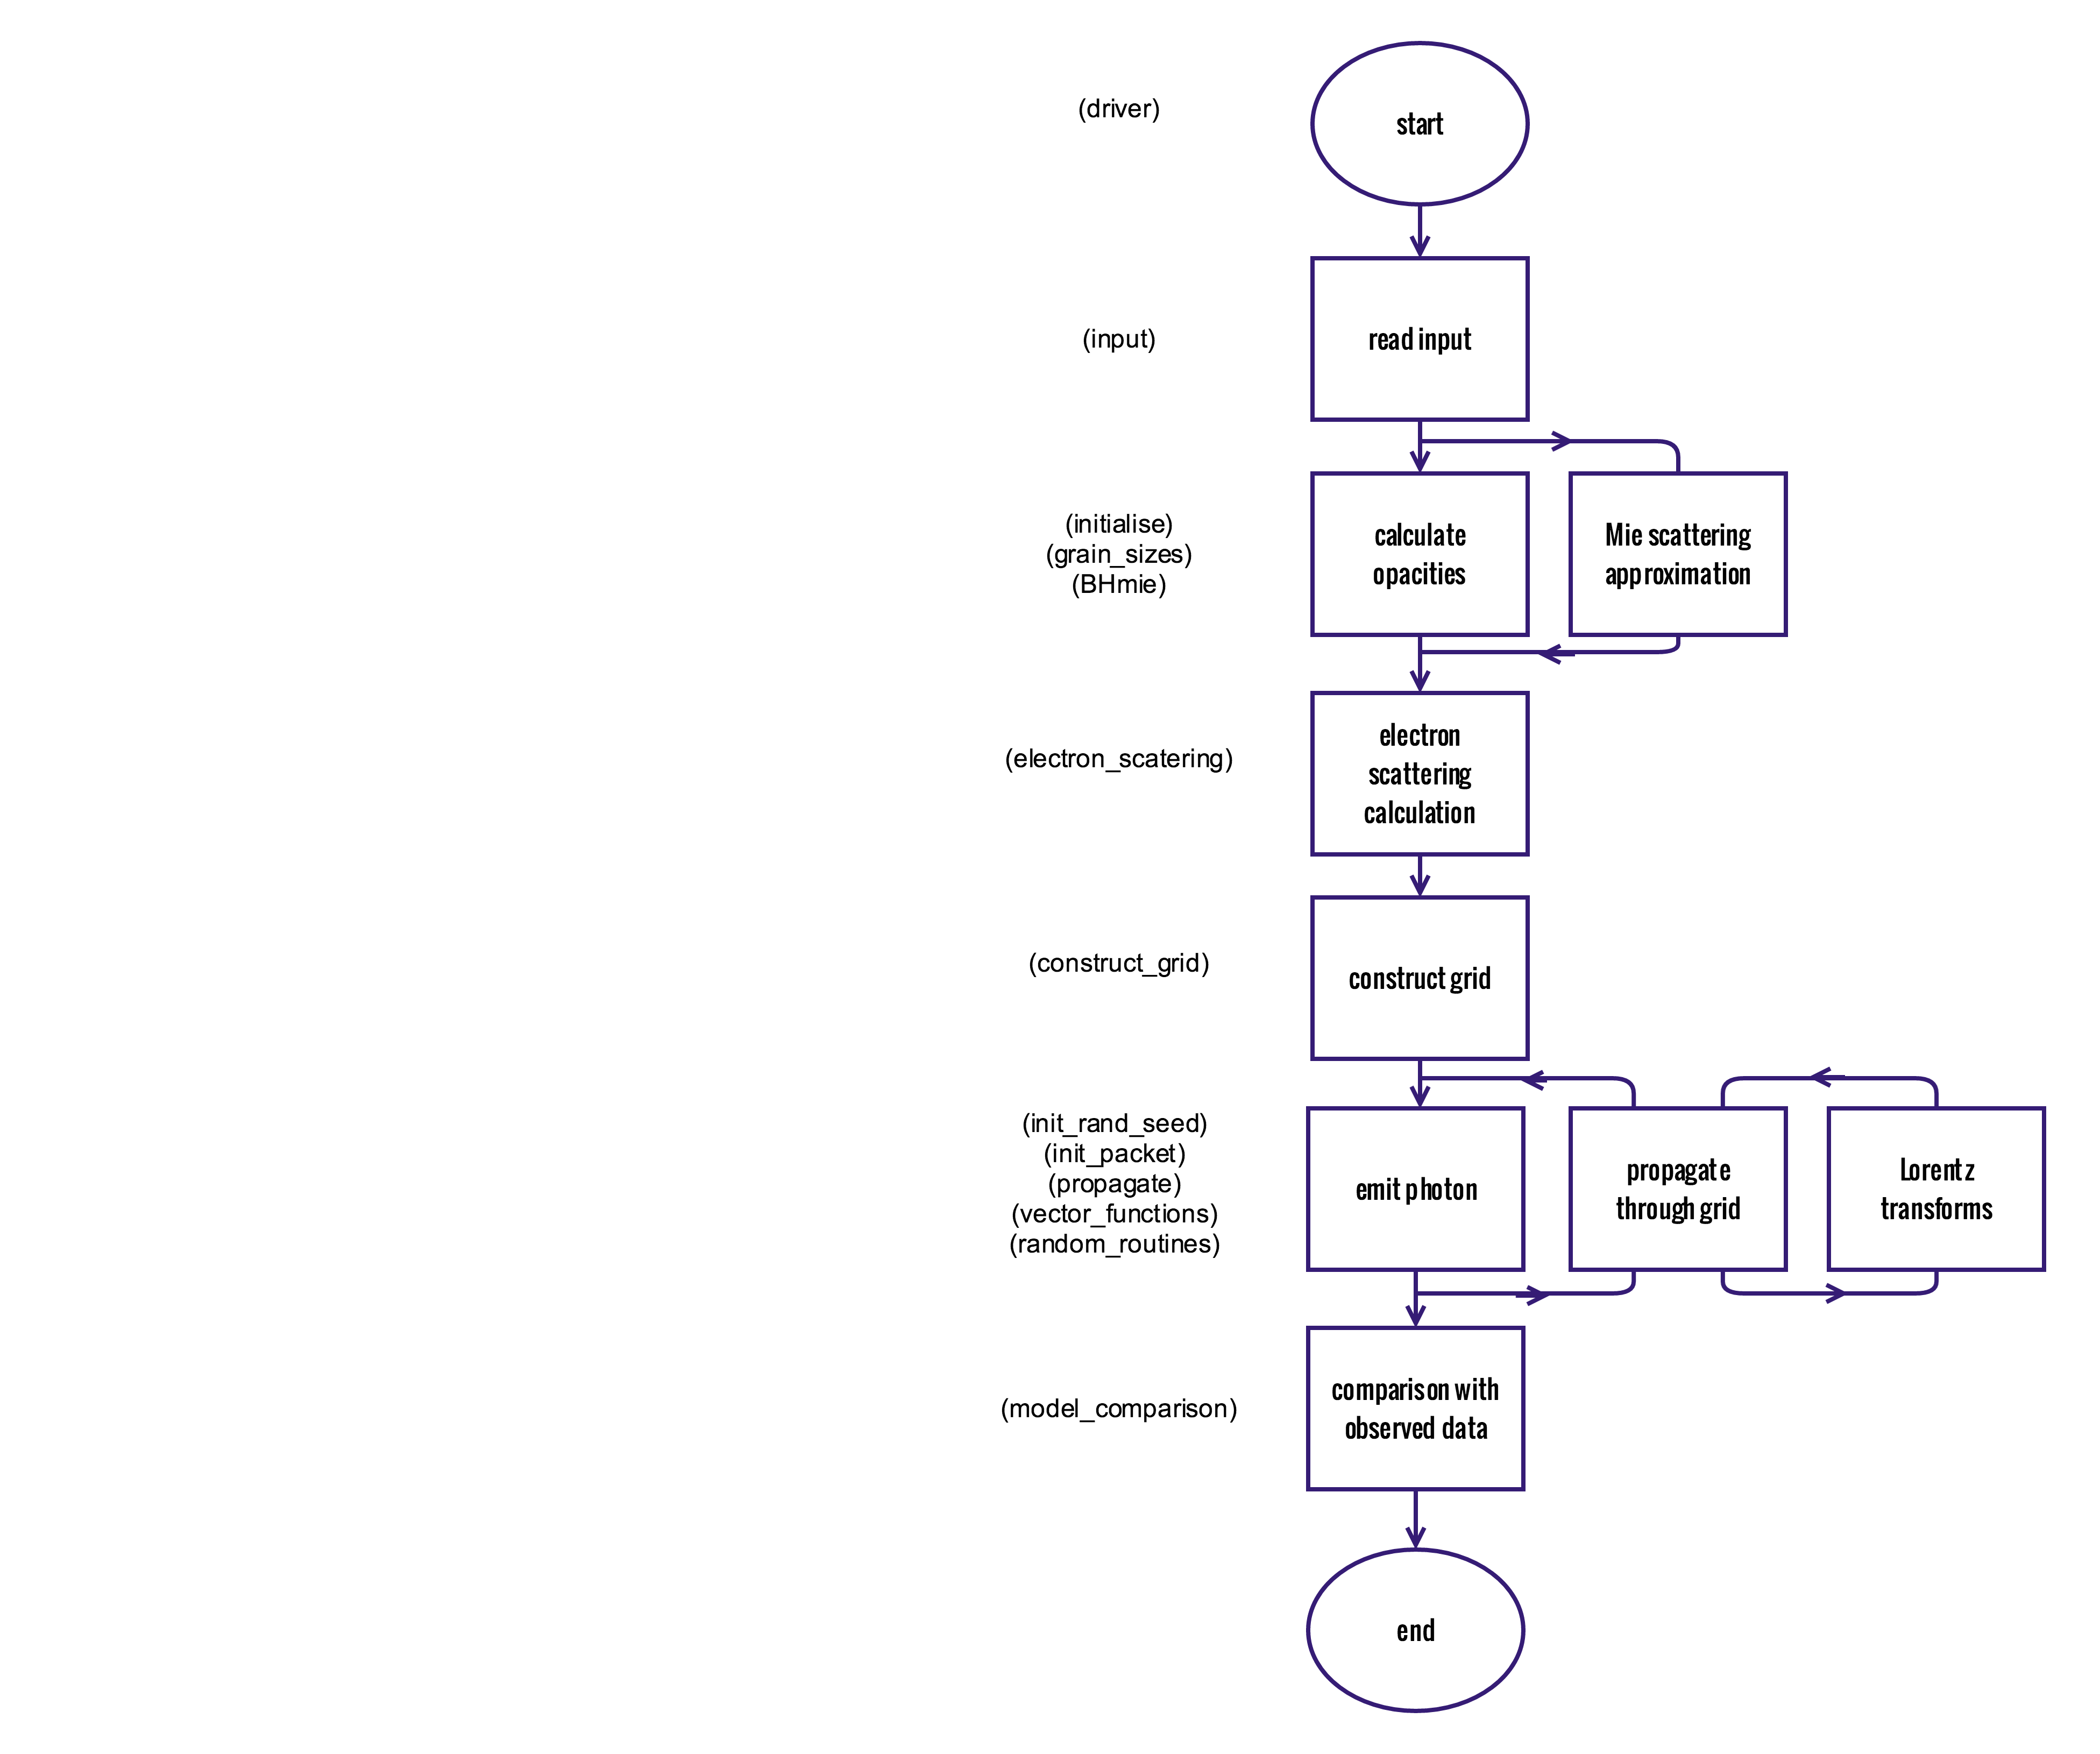
\includegraphics[scale=0.185, trim=650mm 25mm 8mm 25mm]{chapters/chapter2/code_flow.png}
\caption{A flowchart representing the sequence of processes that take place in the DAMOCLES code.  The modules involved at each stage are given in parentheses.}
\label{fig:flowchart}
\end{figure}



\subsection{Energy Packets}

The fundamental principle underlying the Monte Carlo approach to the transport of radiation throughout a dusty nebula is that the radiation is discretised into packets.  Each of these packets is then propagated throughout the nebula and ultimately contributes a fraction of the final energy distribution.  At the start of the simulation, each packet is assumed to consist of $n$ photons of frequency $\nu_0$, the rest frequency of the monochromatic emission line to be modelled.  All packets therefore begin life with initial energy
\begin{equation}
E_0=nh\nu_0
\end{equation}

where $h$ is Planck's constant.  As the packets move through the ejecta, they are scattered off high-velocity dust grains and after each scattering event, the frequency of the packet is altered.  In Monte Carlo simulations that model non-moving atmospheres, packets are usually taken to be of constant energy.  When the frequency of a packet is altered after an event, the energy of that packet is kept constant and the number of real photons contained within it assumed to change.  However, in the case of dust scattering, the number of real photons is conserved and thus the energy of the packet is altered.  This is most easily achieved by weighting each packet over all scattering events as 
\begin{equation}
w_p=\prod_{scat} \frac{\nu'}{\nu}
\end{equation}

\noindent where $w_p$ is the weight of the packet.  The final energy of each packet is then $E =w E_0$, where $E_0$ is the initial energy of the packet.  The final dust-affected line profile is compiled by adding the total energy of all packets in a specific frequency bin in order to produce a histogram.

In these models, unlike fully self-consistent SED radiative transfer models, there is no requirement that the total energy be conserved.  We drop this traditional requirement since radiation that is absorbed by dust is re-emitted outside of the wavelength range of interest and thus no longer contributes any flux to the resulting line profile.  Packets that are absorbed may be safely removed from the simulation.

\subsection{Initialisation and the Grid}

The supernova ejecta is approximated by a three-dimensional cartesian grid, each cell of which is assumed to have uniform density and composition.  By default, the ejecta occupies a shell between inner radius $R_{in}$ and outer radius $R_{out}$. The grid extends from $-R_{out}$ to $+R_{out}$ in each of the three axes.  Each side is split into the same number of divisions and thus each cell is a cube of volume $R_{out}^3/n_{div}^3$ where $n_{div}$ is the number of divisions along each axis and is specified by the user.  For the remainder of this thesis, a spherically symmetric situation is assumed and in all modelling and testing the grid is constructed in this manner.  However, there are no assumptions of symmetry in the code and a cartesian grid was adopted in order to allow for arbitrary geometries to be modelled in the future e.g. ellipsoidal or toroidal ejecta distributions.

\subsubsection{Smooth power-law density distributions}

Both gas and dust are by default assumed to have a power-law distribution declared as  $\rho(r) \propto r^{-\beta}$ between $R_{in}$ and $R_{out}$.  The distribution of gas determines the emissivity distribution and thus the starting positions of the packets in the simulation (see section \ref{sctn:em_prop}).  However, after the initial emission of energy packets, the gas plays no further role in the simulation as only interactions with dust grains are of interest here.  By default, the dust is coupled to the gas and thus follows the same smooth power-law distribution previously described with exponent $-\beta$.  The dust density in each cell is therefore calculated as
\begin{equation}
\rho (r)= \frac{(3-\beta)M_{tot}}{4\pi (R_{out}^{3-\beta}-R_{in}^{3-\beta})} r^{-\beta}
\end{equation}


\noindent if $\beta \neq 3$, where $r$ is the radial distance from the centre of the cell to the origin and $M_{tot}$ is the total desired dust mass to model.  If $\beta = 3$ then the dust density in each cell is alternatively calculated as 
\begin{equation}
\rho (r)= \frac{M_{tot}}{4\pi \log (R_{out}-R_{in})} r^{-3}
\end{equation}

Any cell whose centre falls outside of the bounds of the supernova ejecta has dust density set to zero.  If the dust and gas are decoupled then the user must specify distinct profiles for the gas and the dust; that is, separate power laws must be declared and independent inner and outer radii specified.  The same process is followed but with separate power-laws for each component.  Including the capacity to specify the gas and dust distributions separately allows for more sophisticated modelling of, for example, circumstellar shells or dense cores of dust formation surrounded by more diffuse gas.

\subsubsection{Clumped geometries}

It is known from SED modelling that models of clumped environments produce very different results to environments assumed to have a smooth distribution of dust and gas (e.g. \citet{Bianchi2000,Ercolano2007,Owen2015}).  %Generally, in comparison to smooth models, clumped models tend to require more dust in order to reproduce a similar level of emission or absorption.  
The capacity for modelling a clumped dusty medium is therefore included in the code.  The fraction of the dust mass that is in clumps is declared ($m_{frac}$) and the total volume filling factor of the clumps ($f$) is also specified.  Dust that is not located in clumps is distributed according to a smooth radial power-law.  The clumps occupy  a single grid cell and their size can therefore be varied by altering the number of divisions in the grid.  They are distributed stochastically with probability of a given cell being a clump proportional to the smooth density profile (i.e. $p(r) \propto r^{-\beta}$).  The density of all clumps is constant and is calculated as 
\begin{equation}
\rho_{clump}=\frac{M_{clumps}}{V_{clumps}}=\frac{m_{frac}M_{tot}}{\frac{4}{3} f\pi (R_{out}^{3}-R_{in}^{3} )}
\end{equation}

\noindent where $M_{tot}$ is the total dust mass, $M_{clumps}$ is the total dust mass in clumps and $V_{clumps}$ is the total volume occupied by clumps.  $m_{frac}$ and $f$ are defined as above.

A grid of cubic cells of varying dust and gas densities is thus produced in readiness for packets to be transported through it.  Examples of a smooth and clumped distributions of dust generated by DAMOCLES are presented in Figure \ref{fig:grid}.  A frequency grid is also established centred on the rest-frame frequency of the line to be modelled.



%\begin{figure}
%%		\centering
%\begin{subfigure}{0.4\textwidth}
%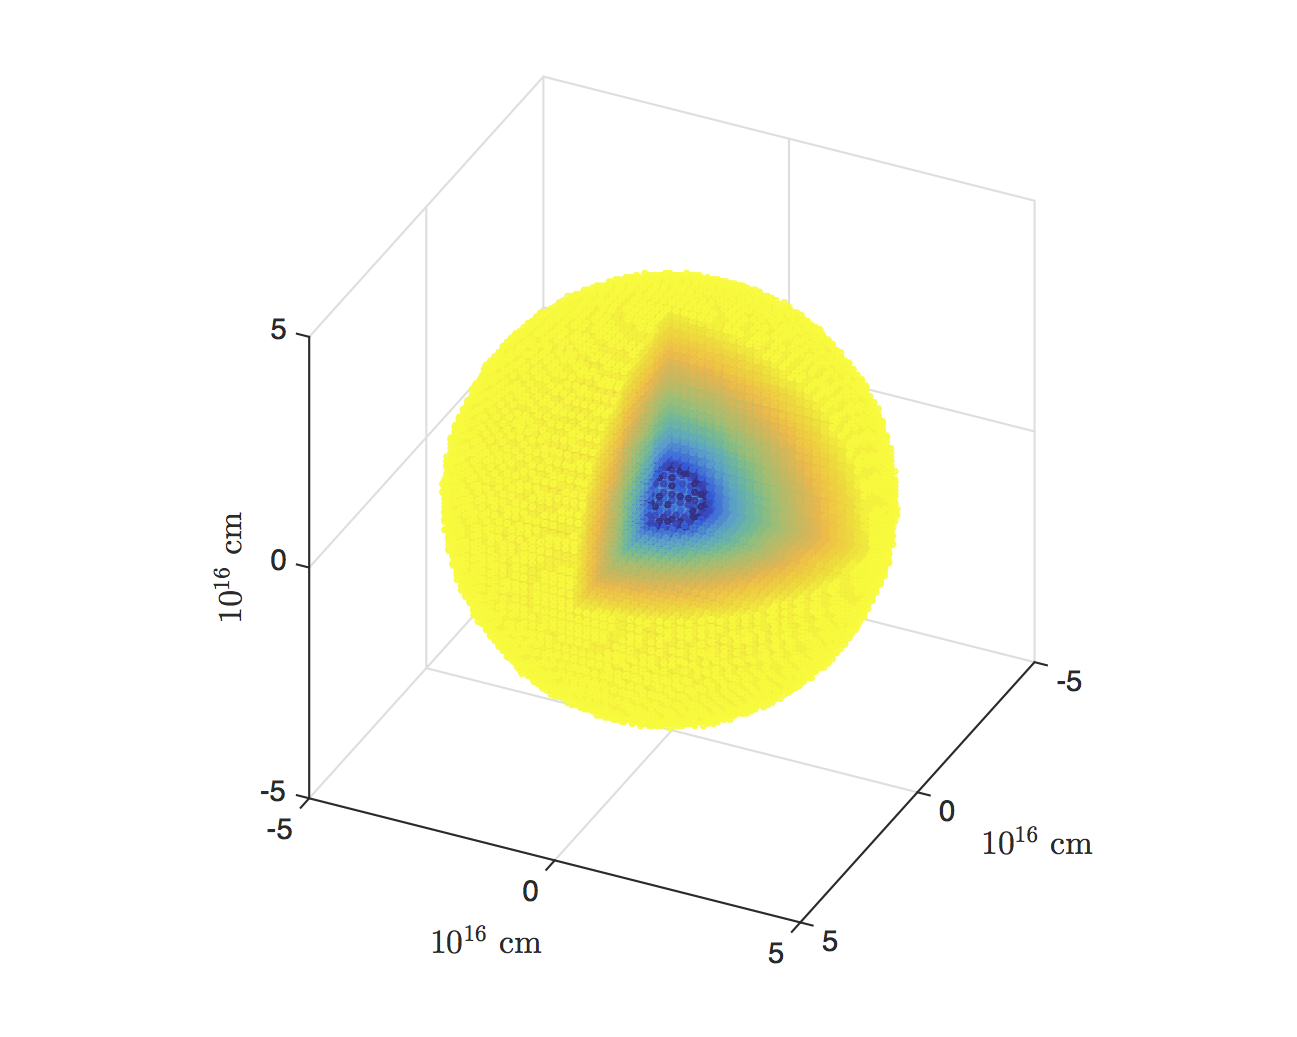
\includegraphics[scale=0.5, trim=35mm 5mm 34mm 5mm,clip=true]{chapters/chapter2/smooth_grid}
%\end{subfigure}
%\hspace{18mm}
%\begin{subfigure}{0.4\textwidth}
%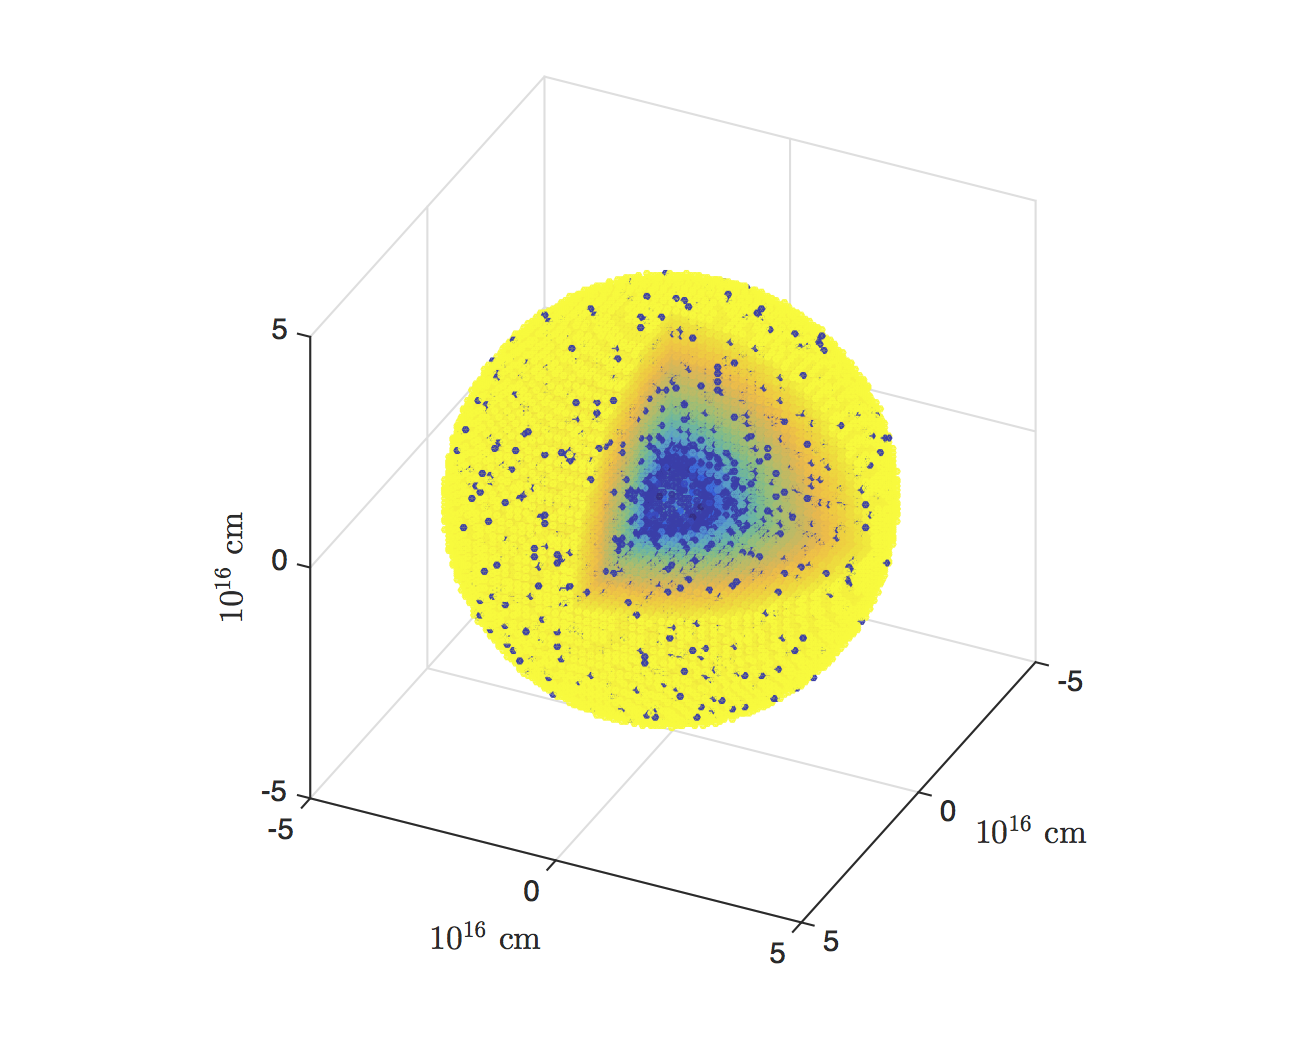
\includegraphics[scale=0.5, trim=35mm 5mm 34mm 5mm,clip=true]{chapters/chapter2/clumped_grid}
%\end{subfigure}
%\caption{3D representations of the grid generated by DAMOCLES.  A smooth distribution is shown on the left and a clumped distribution on the right.}
%\label{fig:grid}
%\end{figure}

%%%%LOW RES VERSION%%%%%%%%
\begin{figure}
%		\centering
\begin{subfigure}{0.4\textwidth}
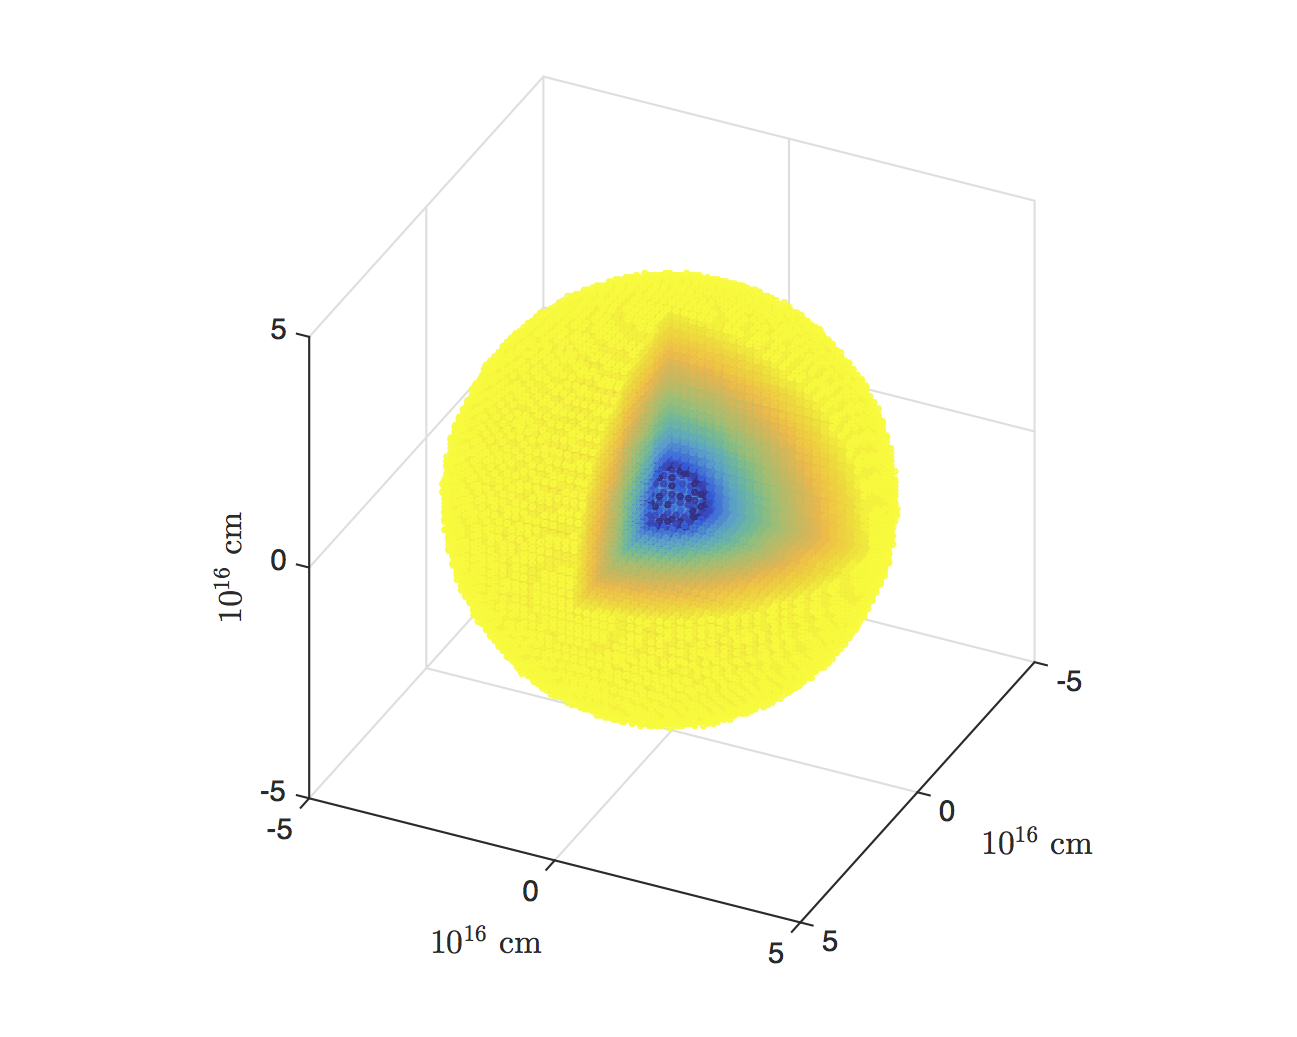
\includegraphics[scale=0.5, trim=35mm 5mm 34mm 5mm,clip=true]{chapters/chapter2/smooth_grid.png}
\end{subfigure}
\hspace{18mm}
\begin{subfigure}{0.4\textwidth}
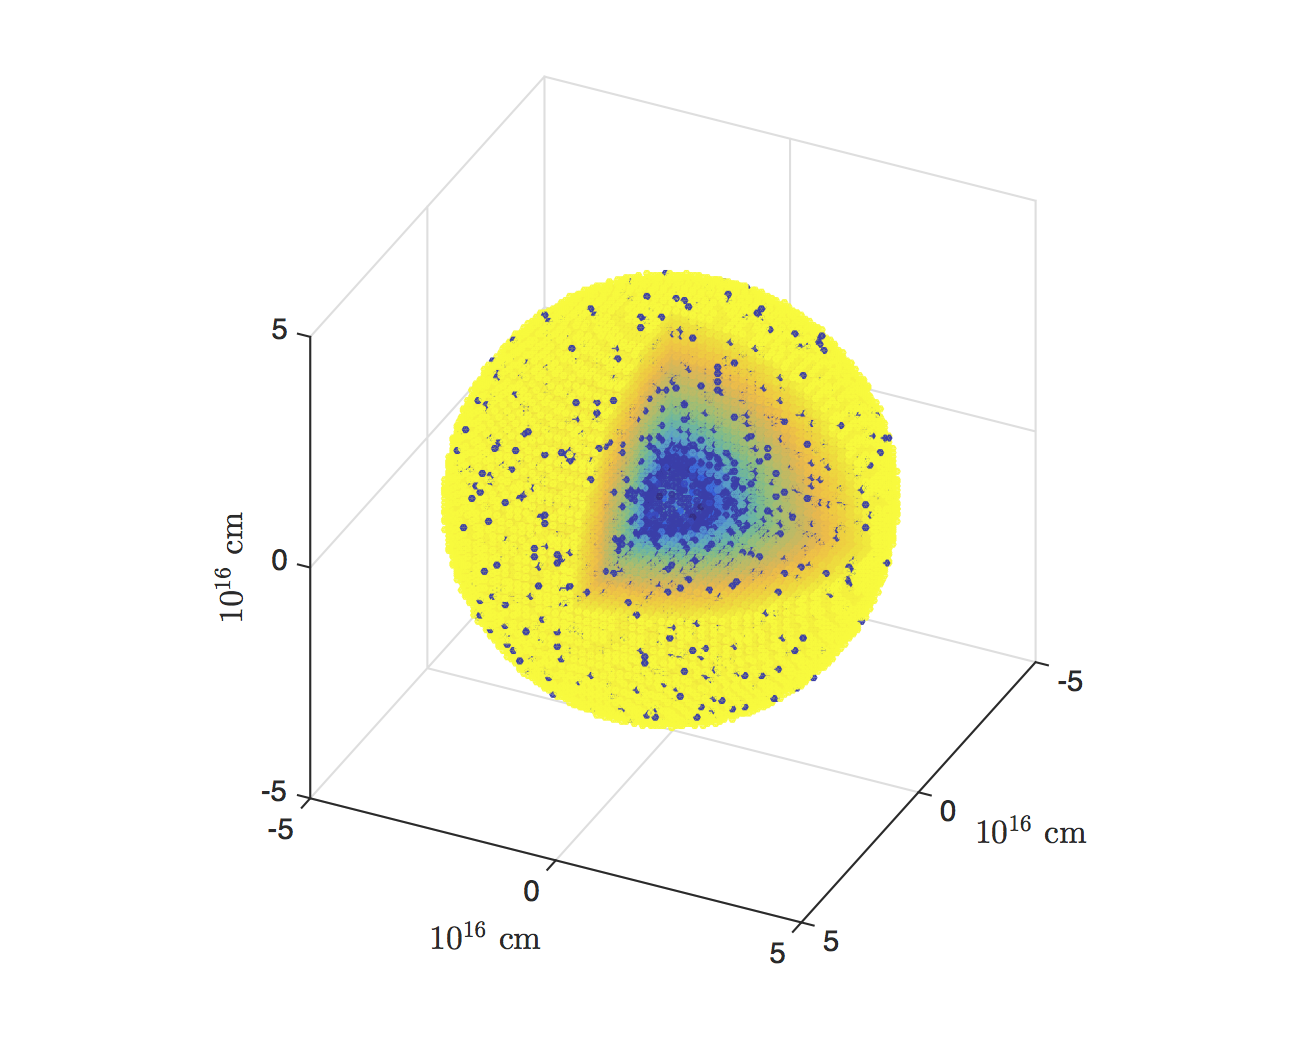
\includegraphics[scale=0.5, trim=35mm 5mm 34mm 5mm,clip=true]{chapters/chapter2/clumped_grid.png}
\end{subfigure}
\caption{3D representations of the grid generated by DAMOCLES.  A smooth distribution is shown on the left and a clumped distribution on the right.}
\label{fig:grid}
\end{figure}


\subsection{Properties of the Dusty Medium}
\label{scn:grainsize}
Dust of any composition may be used for which optical data is available.  The relative abundances of the species must be declared in an input file accompanied by a grain radius distribution (specified as a grain radius range and power-law) for each species.  Files detailing the optical data ($n$ and $k$ values) for the chosen dust species are also declared at the start of the code.  For each pairing of wavelength $\lambda$ and grain radius $a$, a Mie scattering routine is employed to calculate $Q_{abs}(\lambda,a)$ and $Q_{sca}(\lambda,a)$ from the refractive index $n+ik$.  These values are calculated for every species across the wavelength and grain radius ranges of interest.  I have described the mathematics of converting the refractive index into scattering and absorption efficiencies using Mie theory in detail in the introduction to this thesis (see Section \ref{needref}).
%ADD SECTION HERE!!!!


Ultimately, the overall scattering and absorption opacities in each grid cell must be known and so a weighted summation over $Q_{abs}(\lambda,a)$ and $Q_{sca}(\lambda,a)$ is performed.  The number density in each cell must first be calculated as $n = \rho/m_{av}$ where $m_{av}$ is the average mass of a grain: 
\begin{equation}
\label{eqn:Mav}
m_{av}=\sum_i \sum_a \frac{4}{3} \pi a_i^3 \rho_{g,i} w_i(a) x_i
\end{equation}

\noindent $w_i(a)$ represents the normalised weight of particles with grain radius $a$, $\rho_{g,i}$ is the density of the grain for species $i$ (specified with the optical data) and $x_i$ is the relative abundance of species $i$.  

The total cross-section of interaction for extinction is then calculated as
\begin{equation}
\label{eqn:Cext}
C_{ext}(\lambda) = \sum_{i} \sum_a Q_{ext,i}(a,\lambda) w_i(a) \pi a_i^2 x_{i}  
\end{equation}

\noindent where the subscript $i$ denotes species $i$, $x_{i}$ represents the relative abundance of species $i$ and the summations are over species and grain radius.  The calculation of the cross-section of interaction for scattering $C_{sca}(\lambda)$ is performed in the same manner.  

Using equations \ref{eqn:Mav} and \ref{eqn:Cext}, the opacity $\kappa$ can then be calculated using the relationship
\begin{equation}
nC_{ext}=\rho \kappa_{ext}
\end{equation} 

The values of $C_{ext}(\lambda)$ and $C_{sca}(\lambda)$ are calculated for the full wavelength range at the start of the simulation as are the number densities in each grid cell.  As a packet passes through a grid cell, the optical depth $\tau$ is determined from the above quantities according to the wavelength of the current packet (see Section \ref{sctn:em_prop} for further detail on this process).  The above equations are discretised versions of continuous integral equations given in \citet{hulst1957} and \citet{tielens2005}.

%The Mie solution to Maxwell's equations may be approximated under certain conditions to allow for a computationally simple calculation of extinction, scattering and absorption efficiencies.  In particular, this approximation is appropriate in the regime where the wavelength of the incident radiation is of a similar order of magnitude to the diameter of a spherical scatterer.  It is therefore a helpful and suitable approximation to employ in DAMOCLES where we assume dust grains to be approximately spherical and of the order of $\sim 0.1 \mu$m in radius.  Further understanding of the properties of newly-formed dust in the ejecta of supernovae might be obtained by considering alternative approximations for these calculations in future, for example by considering a continuous distribution of ellipsoids in preference to solely spherical grains.  


\subsection{Emission and Propagation}
\label{sctn:em_prop}
The initial radiation field is inherently tied to the distribution of gas throughout the supernova ejecta.  The relationship between the emissivity and the gas density may vary under different regimes and therefore the emissivity distribution is also specified as a power-law with $i(\rho) \propto \rho^{q}$.  In general, however, the emissivity distribution is assumed to be proportional to the square of the local gas density ($i(r) \propto r ^{-2\beta}$), i.e. proportional to the product of the recombining 
ion and electron densities in the case of a recombination line or to the product of the neutral atoms and electron densities in the case of collisionally excited line emission.

The supernova ejecta is divided into shells between $R_{in}$ and $R_{out}$ and the number of packets to be emitted in each shell calculated according to the specified power-law emissivity distribution $i(r) \propto r^{-q\beta }$.  For each packet a location within the appropriate shell must be determined and a propagation direction sampled.  The initial propagation direction is sampled from an isotropic distribution as detailed in numerous publications (e.g. \citet{Wood2004}). Three random numbers in the range $[0,1)$ are sampled and these are translated into spherical coordinates as 
%\begin{equation}
\begin{align}
\label{eqn:isotropic}
\phi&=2\pi\eta \\
\theta&=\arccos(2\xi -1) 
\end{align}
%\end{equation}

\noindent where $\eta$ and $\xi$  are random numbers in the range $[0,1)$, $\phi$ is the azimuthal angle and $\cos \theta$ is the radial direction cosine.  The initial packet trajectory in cartesian is then given by 
\begin{align}
n_x&=\sin\theta\cos\phi \\
n_y&=\sin\theta\sin\phi \\
n_z&=\cos\phi
\label{eqn:isotropic2}
\end{align}

The process for sampling an initial position within the shell follows the same sampling process as described above  but a radial position must be sampled in addition to the two angular coordinates.  For a random number $\zeta$, the radial position $r$ is calculated as
\begin{equation}
r=R_i+\zeta(R_{i+1}-R_i)
\label{eqn:isotropic3}
\end{equation}
\noindent where $R_i$ is the inner boundary of the $i$\textsuperscript{th} shell.

In total therefore five random numbers must be sampled in order to generate an initial position and trajectory for a packet. At every subsequent scattering event, the packet is propelled with a new direction vector which is sampled from an isotropic distribution in the rest-frame of the particle with two newly generated random numbers in the manner described above.  I do not include forward-scattering matrices in the code since the effects of forward scattering by dust are so small as to be negligible and it is simpler and more efficient simply to assume isotropic scattering.  

Once a packet has been emitted into the nebula, it must be propagated through the grid until it escapes the outer bound of the ejecta $R_{out}$ or is absorbed.  In each cell that a packet passes through, a test must be performed in order to determine whether the packet passes through that cell and into the next or whether it is scattered or absorbed by a dust grain (i.e. an ``event" occurs).  The probability that a packet travels a distance $l$ without interacting is 
\begin{equation}
p(l)=e^{-n \sigma_{\lambda} l}=e ^{-\tau_{\lambda}} 
\end{equation}

\noindent where $n$ is the number density of the grid cell, $\sigma_{\lambda}$ is the cross-section of interaction at wavelength $\lambda$ and 
\begin{equation}
\tau_{\lambda} = n\sigma_{\lambda} l = \rho \kappa_{\lambda}  l
\end{equation}

\noindent for constant $n$ and $\sigma_{\lambda}$ (as in a grid cell).  Note that $\sigma_{\lambda}$ is used to denote the cross-section of interaction for a given grain radius.  Where a grain radius distribution is adopted or multiple species are employed, the formula becomes $\tau_{\lambda} = nC_{ext,\lambda}l$ as described in Section \ref{scn:grainsize}.  The probability that a packet \textit{does} interact within a distance $l$ is therefore $1-e^{-\tau_{\lambda}}$.  The position at which the packet will be absorbed or scattered is then determined by comparing a randomly generated number in the interval [0,1) with this value.  In practice however, it is easier to sample from the cumulative probability distribution and use the generated number to calculate an optical depth as 
\begin{equation}
\xi = 1 - e^{-\tau_{\lambda}}  \implies  \tau_{\lambda}=-\log (1-\xi) 
\end{equation}

\noindent where $\xi \in [0,1)$ is a sampled random number between $0$ and $1$.  The properties of the cell as determined in Section \ref{scn:grainsize} are then used to determine the distance that the packet travels:
\begin{equation}
l=\frac{\tau_\lambda}{nC_{ext,\lambda}}
\end{equation}

 If the distance to be travelled by the packet is greater than the distance from its position to the edge of the cell then the packet is moved along its current trajectory $(n_x,n_y,n_z)$ to the cell boundary and the process is repeated.  Alternatively, if the displacement is not sufficient for the packet to escape the cell then an event occurs.  The packet is either scattered or absorbed with probability of scattering equal to the albedo of the cell
\begin{equation}
\omega=\frac{\sigma_{sca}}{\sigma_{sca}+\sigma_{abs}}
\end{equation}

If the packet is absorbed (the case if a randomly generated number is greater than the albedo $\omega$) then it is simply removed from the simulation as previously discussed.  If this is not the case, then the packet is scattered and a new trajectory is sampled from an isotropic distribution in the comoving frame of the dust grain.  The frequency of the packet is recalculated using Lorentz transforms as described in the next section and the process is repeated until the packet has either escaped the outer boundary of the supernova ejecta or been absorbed.  If the packet does escape, its weighted energy is deposited in the appropriate frequency bin.  Once all packets have escaped, the array of frequencies and fluxes produces the desired line profile.

\subsection{The Velocity Field and Doppler shifting}

At emission and at each scattering event the frequency of the packet is recalculated according to a radial velocity field 
\begin{equation} 
v(r) = v_{max}\frac{r^{\alpha}}{R_{out}^{\alpha}}
\end{equation}

\noindent where the maximum velocity, $v_{max}$, at the outer edge of the ejecta and the exponent of the velocity profile, $\alpha$, are declared in the input file.	

It is worth noting that if a constant mass loss rate is required, the exponent of the velocity profile and the exponent of the density profile are not independent.  A constant mass loss rate implies that $4\pi \rho vR^2  \propto k$, where $k$ is a constant, and thus for $v \propto r^\alpha$ and $\rho\propto r^{-\beta}$, we require that $\beta-\alpha=2$.  However, it is possible that the supernova event may have induced a mass-flow rate that is not constant with radius and thus both exponents may be declared independently.  It is also worth noting that for supernovae in their free expansion phase, as the majority are by the time of the onset of dust formation, the ejecta are expanding with a $v \propto r$ Hubble law expansion.

The outflow velocities in supernovae are extremely high, of the order of 10\% of the speed of light.  Escaping radiation is therefore subject to significant Doppler shifting. At emission and at each scattering event, the frequency of a packet must be recalculated according to the velocity of the scattering or emitting grain.  When the packet is initially emitted, it has a frequency and a trajectory in the rest frame of the emitter. Both of these must be transformed to the observer's frame in order for the packet to be propagated through the grid.  The new direction and frequency in the observer's frame may be simply found by transforming the momentum 4-vector $\boldsymbol{P}$ which is defined as
\begin{equation}
\boldsymbol{P}=
\begin{pmatrix}
E \\
p_x \\
p_y \\
p_z \\
\end{pmatrix} =
\begin{pmatrix}
h \nu \\
h \nu x \\
h \nu y \\
h \nu z \\
\end{pmatrix}
\end{equation}


\noindent We may then derive $\boldsymbol{P'}$, the momentum 4-vector in the observer's frame using the relation
\begin{equation}
\boldsymbol{P'}=\Lambda \boldsymbol{P}	
\end{equation}

\noindent where 
\begin{equation}
{\Lambda}=
\begin{pmatrix} 
\gamma & -\gamma \beta_x & -\gamma \beta_y & -\gamma \beta_z \\
-\gamma \beta_x & 1+(\gamma-1)\frac{\beta_x^2}{\beta^2} & 
(\gamma-1)\frac{\beta_x \beta_y}{\beta^2} & (\gamma-1)\frac{\beta_x \beta_z}{\beta^2} \\
-\gamma \beta_y  & (\gamma-1)\frac{\beta_y \beta_x}{\beta^2} & 1+(\gamma-1)\frac{\beta_y^2}{\beta^2} 
& (\gamma-1)\frac{\beta_y \beta_z}{\beta^2}\\
-\gamma \beta_z & (\gamma-1)\frac{\beta_z \beta_x}{\beta^2} & (\gamma-1)\frac{\beta_z \beta_y}{\beta^2} 
& 1+(\gamma-1)\frac{\beta_z^2}{\beta^2} \\
\end{pmatrix}
\\
\end{equation}
\\
\\
\noindent and $\boldsymbol{\beta}=\frac{{\bf{v}}}{c}=(\beta_x,\beta_y,\beta_z)$,   $\beta=\lvert \boldsymbol{\beta}\rvert$ and $\gamma = \frac{1}{\sqrt{1-\beta^2}}$.
\\

In practice, the velocities considered are low enough that it is unnecessary to consider terms of order $O(\frac{v^2}{c^2})$ and thus ${\Lambda}$ may be reduced to
\begin{equation}
{\Lambda}=
\begin{pmatrix} 
1 & - \beta_x & - \beta_y & - \beta_z \\
- \beta_x & 1 & 0 & 0 \\
- \beta_y  & 0 & 1 & 0\\
- \beta_z & 0 & 0 & 1 \\
\end{pmatrix}
\\
\end{equation}

\noindent The new direction of travel and frequency in the observer's frame are therefore given by  
\begin{equation}
\nu'=\nu(1-x\beta_x-y\beta_y-z\beta_z) \\
\end{equation}
\begin{equation*}
\begin{split}
x'=\frac{\nu}{\nu'}(x-\beta_x) \\
y'=\frac{\nu}{\nu'}(x-\beta_y) \\
z'=\frac{\nu}{\nu'}(x-\beta_z) \\
\end{split}
\end{equation*}

For each scattering event, the packet must be transformed both into and out of the comoving frame. The reverse transform is applied by using the inverse Lorentz matrix $\Lambda^{-1}$ which is obtained by reversing the sign of $\bf{v}$.  Positive $\bf{v}$ is defined for frames moving away from each other and thus $\bf{v}$ is defined to be negative in the direction of the observer.

\begin{table}[htdp]
\caption{Values of $q_{H\alpha}(T)$ at three different temperatures as used by DAMOCLES.}
\begin{center}
\def\arraystretch{1.5}
\begin{tabular}{ c c c c}
\toprule
&&Temperature (K) & \\
\cmidrule{2-4}
& 5,000 & 10,000 & 20,000  \\
\midrule
$q_{H\alpha}$ (erg cm$^3$ s$^{-1}$)  & $6.71\times 10^{-25}$	&$3.56\times 10^{-25}$	&$1.83\times 10^{-24}$  \\
\bottomrule
\end{tabular}
\end{center}
\label{tb:q}
        \end{table}%

        \subsection{Electron Scattering}
        \label{scn:ES}

        As will be discussed in detail in chapter three, the effects of scattering on the shapes of line profiles can be quite pronounced and it is therefore important to consider the potential effects of electron scattering as well as those of dust scattering.  A simple treatment of electron scattering calculates electron densities using an estimated average temperature of either 5,000K, 10,000K or 20,000K.  An observed luminosity of $H{\alpha}$ is then used to calculate the optical depth to electrons.  The overall optical depth within each cell is calculated as $\tau = \tau_{dust}+\tau_{e}$, with $\tau_{e}=0$ if electron scattering is not activated.  The electron scattering optical depth, $\tau_e$, in a given cell (with constant properties therein) is calculated as 
        \begin{equation}
        \tau_e =  n_e \sigma_t l
        \end{equation}
        
        \noindent where $n_e$ is the electron density in that cell,  $\sigma_t$ is the Thomson cross-section of interaction for an electron and $l$ is the distance travelled.	
        In order to calculate this value, the electron density in each cell must be known.  We assume that the electron density is the same as the proton density and that both are distributed according to the gas density distribution such that 
        \begin{equation}
        \label{eqn:es_distn}
        n_e(r) = Kr^{-\beta}
        \end{equation}

        \noindent  where $K$ is a constant.  The value of $K$ must be determined from the total H$\alpha$ luminosity.  We follow the formalism described by \citet{Osterbrock2006} in order to estimate the electron density from the total H$\alpha$ luminosity ($L_{H\alpha}$). $L_{H\alpha}$ is given by
        \begin{align}
        L_{H\alpha} =& \int _0 ^{\infty} n_p(r) n_e(r) E_{H\alpha} \alpha^{eff}_{H\alpha}(T) ~ \, 4 \pi r^2 \, dr  \\
        =& \int _{R_{in}} ^{R_{out}} n_p(r) n_e(r) q_{H\alpha}(T) ~ \, 4 \pi r^2 \, dr \label{eqn:es_lum}
        \end{align}

        \noindent where $n_p(r)$ is the proton density at radius $r$, $n_e(r)$ is the electron density at radius $r$, $T$ is the temperature, $\alpha^{eff}_{H\alpha}(T)$ is the temperature-dependent effective recombination coefficient for H$\alpha$, $E_{H\alpha}$ is the energy of a single H$\alpha$ photon and 
        \begin{equation}
        q_{H\alpha}=E_{H\alpha} \alpha^{eff}_{H\alpha}=\frac{4 \pi j_{H\alpha}}{n_e n_p}
        \end{equation}

        \noindent where $j_{H\alpha}$ is the temperature-dependent emission coefficient for H$\alpha$ (i.e. the energy emitted per unit volume per unit time per unit solid angle).  Substituting equation \ref{eqn:es_distn} into equation \ref{eqn:es_lum} gives the following
        \begin{equation}
        \frac{L_{H\alpha}}{4 \pi q_{H\alpha}} = k^2 \int _{R_{in}} ^{R_{out}} r^{2(1-\beta)} \, dr
        \end{equation}

        which in the case $\beta \ne \frac{3}{2}$ may be solved as 
        \begin{equation}
        \label{eqn:kcalc1}
        K= \sqrt{\frac{L_{H\alpha}}{4 \pi q_{H\alpha}} ~\frac{3-2\beta}{R_{out}^{3-2\beta}-R_{in}^{3-2\beta}}}
        \end{equation}

        and for $\beta=\frac{3}{2}$ is
        \begin{equation}
        \label{eqn:kcalc2}
        K= \sqrt{\frac{L_{H\alpha}}{4 \pi q_{H\alpha}} ~\frac{1}{\ln({R_{out}/R_{in}})}}
        \end{equation}

        Substituting $K$ back into equation \ref{eqn:es_distn} gives the electron density for each cell.  In the code, only three gas temperatures may be specified and three corresponding values of $q_{H\alpha}(T)$ are included as per Table \ref{tb:q}.


        If, for a given packet, an event occurs, it is first calculated whether this is an electron scattering event or a dust event (either scattering or absorption) by considering the ratio of the optical depths to each. The process by which a packet is scattered by an electron is almost identical to the dust scattering process except for the adopted velocity of the scatterer.  In the case of a dust grain, the velocity is simply the bulk velocity of the ejecta at that radius as determined from the specified velocity profile.  For an electron, the assumed velocity must include a thermal component as well as the same bulk velocity as would be adopted for a dust grain at the same location.  As per the electron scattering calculation of \citet{Hillier1991}, the components $(v_x,v_y,v_z)$ of the thermal velocity $\boldsymbol{v}_{therm}$ are assumed to follow a Maxwellian distribution with zero mean and standard deviation 
        \begin{equation}
        \label{eqn:sigma_maxwell}
        \sigma=\sqrt{\frac{k_BT}{m_e}}
        \end{equation}

        \noindent where $k_B$ is Boltzman's constant and $m_e$ is the mass of an electron.  The components are then sampled from a normal distribution with specified mean and standard deviation using the Marsaglia polar method \citep{Marsaglia1964}.  This method generates two random numbers from a uniform distribution in the interval [0,1) and uses a number of transformations to convert them to random numbers as generated from a standard normal distribution with zero mean and unity variance.  They may then be scaled to the appropriate normal distribution.  Finally, the overall velocity of the electron is then calculated as 
        \begin{equation}
        \boldsymbol{v}_e=\boldsymbol{v}_{bulk}+\boldsymbol{v}_{therm}
        \end{equation}

        and the Lorentz transforms are applied in the same manner as a dust scattering event.

        In the majority of cases it seems that the electron densities are not high enough to discernibly effect the overall shape of the profile.  However, there may be a few rare cases (the concept is discussed for SN 2010jl \citep{Fransson2013}) where the electron densities are high enough to become significant in the observed profiles.  Whilst the inclusion of electron scattering in the code is an approximation since it is not necessarily true that $n_e=n_p$ and the exact gas temperature is unknown, it gives a good suggestion of the potential effects of electron scattering.	
        
        \subsection{Doublets}

        One of the lines in supernovae emission spectra that is frequently seen to be blue shifted is the forbidden [OI]$\lambda$6300,6363\AA\ doublet.  DAMOCLES therefore has the capacity to treat doublets as well as single lines.  When a doublet is specified, both the initial wavelengths and the initial intensity ratio must be declared.  The code will create a wider frequency array than for a single line in order to accommodate both lines.  It will then model each line independently, adding the final fluxes of the lines weighted by their intrinsic flux ratio to produce the desired doublet at the end of the modelling. 

        \subsection{Comparing the Model with Observations}

        DAMOCLES includes the capacity to read in observed line profile data for direct comparison with a modelled line profile.  Once all packets have been processed through the nebula and collected into bins, a flux is calculated at each of the wavelength bins in the observed data by interpolating between modelled wavelength bins.  A mean squared error (MSE) calculation is then performed to compare the model with the data quantitatively, where the MSE is equal to	
        \begin{equation}
        \label{eqn:chi2}
        \frac{1}{N} \sum_i (f_{obs,i}- f_{mod,i})^2
        \end{equation}		
        
        \noindent and $f_{obs,i}$ is the observed flux in the $i$\textsuperscript{th} frequency bin, $f_{mod,i}$ is the modelled flux in the $i$\textsuperscript{th} frequency bin, and $N$ is the total number of frequency bins.   Minimising the MSE minimises the error between the model and the observed line and therefore provides a quantitative measure of goodness of fit that may be used in addition to or instead of any qualitative assessment.  Since the total inherent error on each observation is variable, the exact value of the MSE should not be compared between different line profile observations and only between different models and sets of parameters for a given line profile.
        
        \section{The Structure of DAMOCLES}
        \label{damocles_struct}
        
        DAMOCLES is written using Fortran 95.  Since the major modernisation of Fortran 77 in 1990, the language includes a number of more modern elements that make it an ideal choice for this type of numerical computation.  Firstly, a fast, high-level language is required that allows for dynamic memory allocation and deallocation.  Whilst DAMOCLES could have been written in a number of other languages, this is a critical feature that is only available in a few languages.  Very large numbers of packets are required to achieve reasonable resolutions in Monte Carlo codes of this nature and therefore  large arrays of data are required.  The ability to maintain careful control of memory allocation is very important.  
        
        Fortran 95 also has a number of other features that make it especially suitable for this sort of code.  Derived types group a number of variables of different intrinsic or other derived types.  This allows different properties of a particular item (for example a packet or grid cell) to be grouped together and accessed via that item. Though not a necessary feature, derived types make the code simpler, faster and more legible.  They also make it easier to write and therefore help to minimise the risk of errors.  Similarly, the modular structure that was introduced to Fortran in 1990 allows the programmer to distribute their code over a number of modules and ensures that variables that are declared within a particular module can be accessed by other modules if necessary \citep{Ellis1994}.  This eliminates the need for common blocks of code and allows a large program to be segmented into logical divisions.  This increases the speed, clarity and ease of maintenance and development in the future.
        
        The obvious alternative programming language to Fortran 95 is C or C++.  Both of these languages have all of the features described above and are exceptionally fast.  From a computation perspective, there is, arguably, little to separate them for this type of coding.  I ultimately decided to write DAMOCLES in Fortran 95 because of its heritage in astrophysics.  A very large number of astrophysical codes have been written using current or previous versions of Fortran and writing the code in Fortran 95 allowed for easy compatibility and the use of various astrophysics libraries and routines.
        
        DAMOCLES is parallelised using OpenMP (see Section \ref{scn:open_mp}) which restricts its use to shared memory machines.  It has been developed on and currently runs on a MacBook Pro 11.2 quad core with Intel Core i7 2.8GHz processors and 16GB of memory.  A typical, medium resolution simulation using 125,000 grid cells and 10$^5$ packets takes approximately 15 seconds to run.  The number of packets transported and the total dust optical depth are the most important factors in determining runtime.  	

        
        \subsection{Computational Architecture and Processes}
        DAMOCLES was written using a modular structure.  The ``parent" driver has numerous ``children" in the form of subroutines and modules which are each responsible for a separate task or tasks.  This architecture has a number of advantages.  Firstly, it serves to clarify both the functionality and legibility of the code allowing for easier debugging and maintenance.  It also allows for the implementation of features such as recursive subroutines which are ideally suited to a Monte Carlo methodology.  Finally, it allows for the code to be developed further in the future simply by including additional modules and subroutines.  A brief description of every module and subroutine in the code is presented in the following subsections.  The descriptions are ordered according to the first time they or their contents are called by the driver (see Figure \ref{fig:flowchart} for a flowchart of the order of the processes that take place in DAMOCLES and see Figure \ref{fig:flowchart_mods} for a flowchart of the modular hierarchy).
        

        \subsubsection{The driver}
        The \textit{driver} module is at the centre of DAMOCLES.  It is from here that all subroutines are called.  The calls to construct the grid and calculate dust opacities, to emit and propagate packets and to compare the results with observational data are all made from here.  The parallelisation process is also controlled from here (see section \ref{scn:open_mp} for more details on the parallel function of DAMOCLES).  Having called the initialisation routines, the driver is responsible for dividing the ejecta into shells and calculating how many packets are emitted within each shell.  Each shell is looped over and each packet is looped over within each shell. Emission and propagation routines are called inside this loop.  At the end of each packet's lifetime, either once it has been absorbed or has escaped, the driver adds the weighted packet's energy to the appropriate frequency bin and stores this information before looping back to emit and propagate the next packet.  It is here that a line of sight is applied if so desired.  This is achieved by collecting only packets that have escaped within a cone of vertical angle $\pi/6$.  Once all packets have been processed, the driver writes the relevant information (the wavelengths, velocities and fluxes that describe the outputted line profile) to an output file and calls the model comparison module.  
        
        The driver is also the section of code responsible for processing doublets.  The code treats doublets by processing two batches of packets with differing initial frequency through the same grid.  Before they are collected in frequency bins, the flux ratio that is specified by the user is applied to one batch of the packets.  All packets are then collected as per a single line. 
        
        Various statistics are also processed and output here including the fraction of packets that are absorbed and the estimated undepleted luminosity of the observed line. 
        

        \begin{figure}
        \centering
        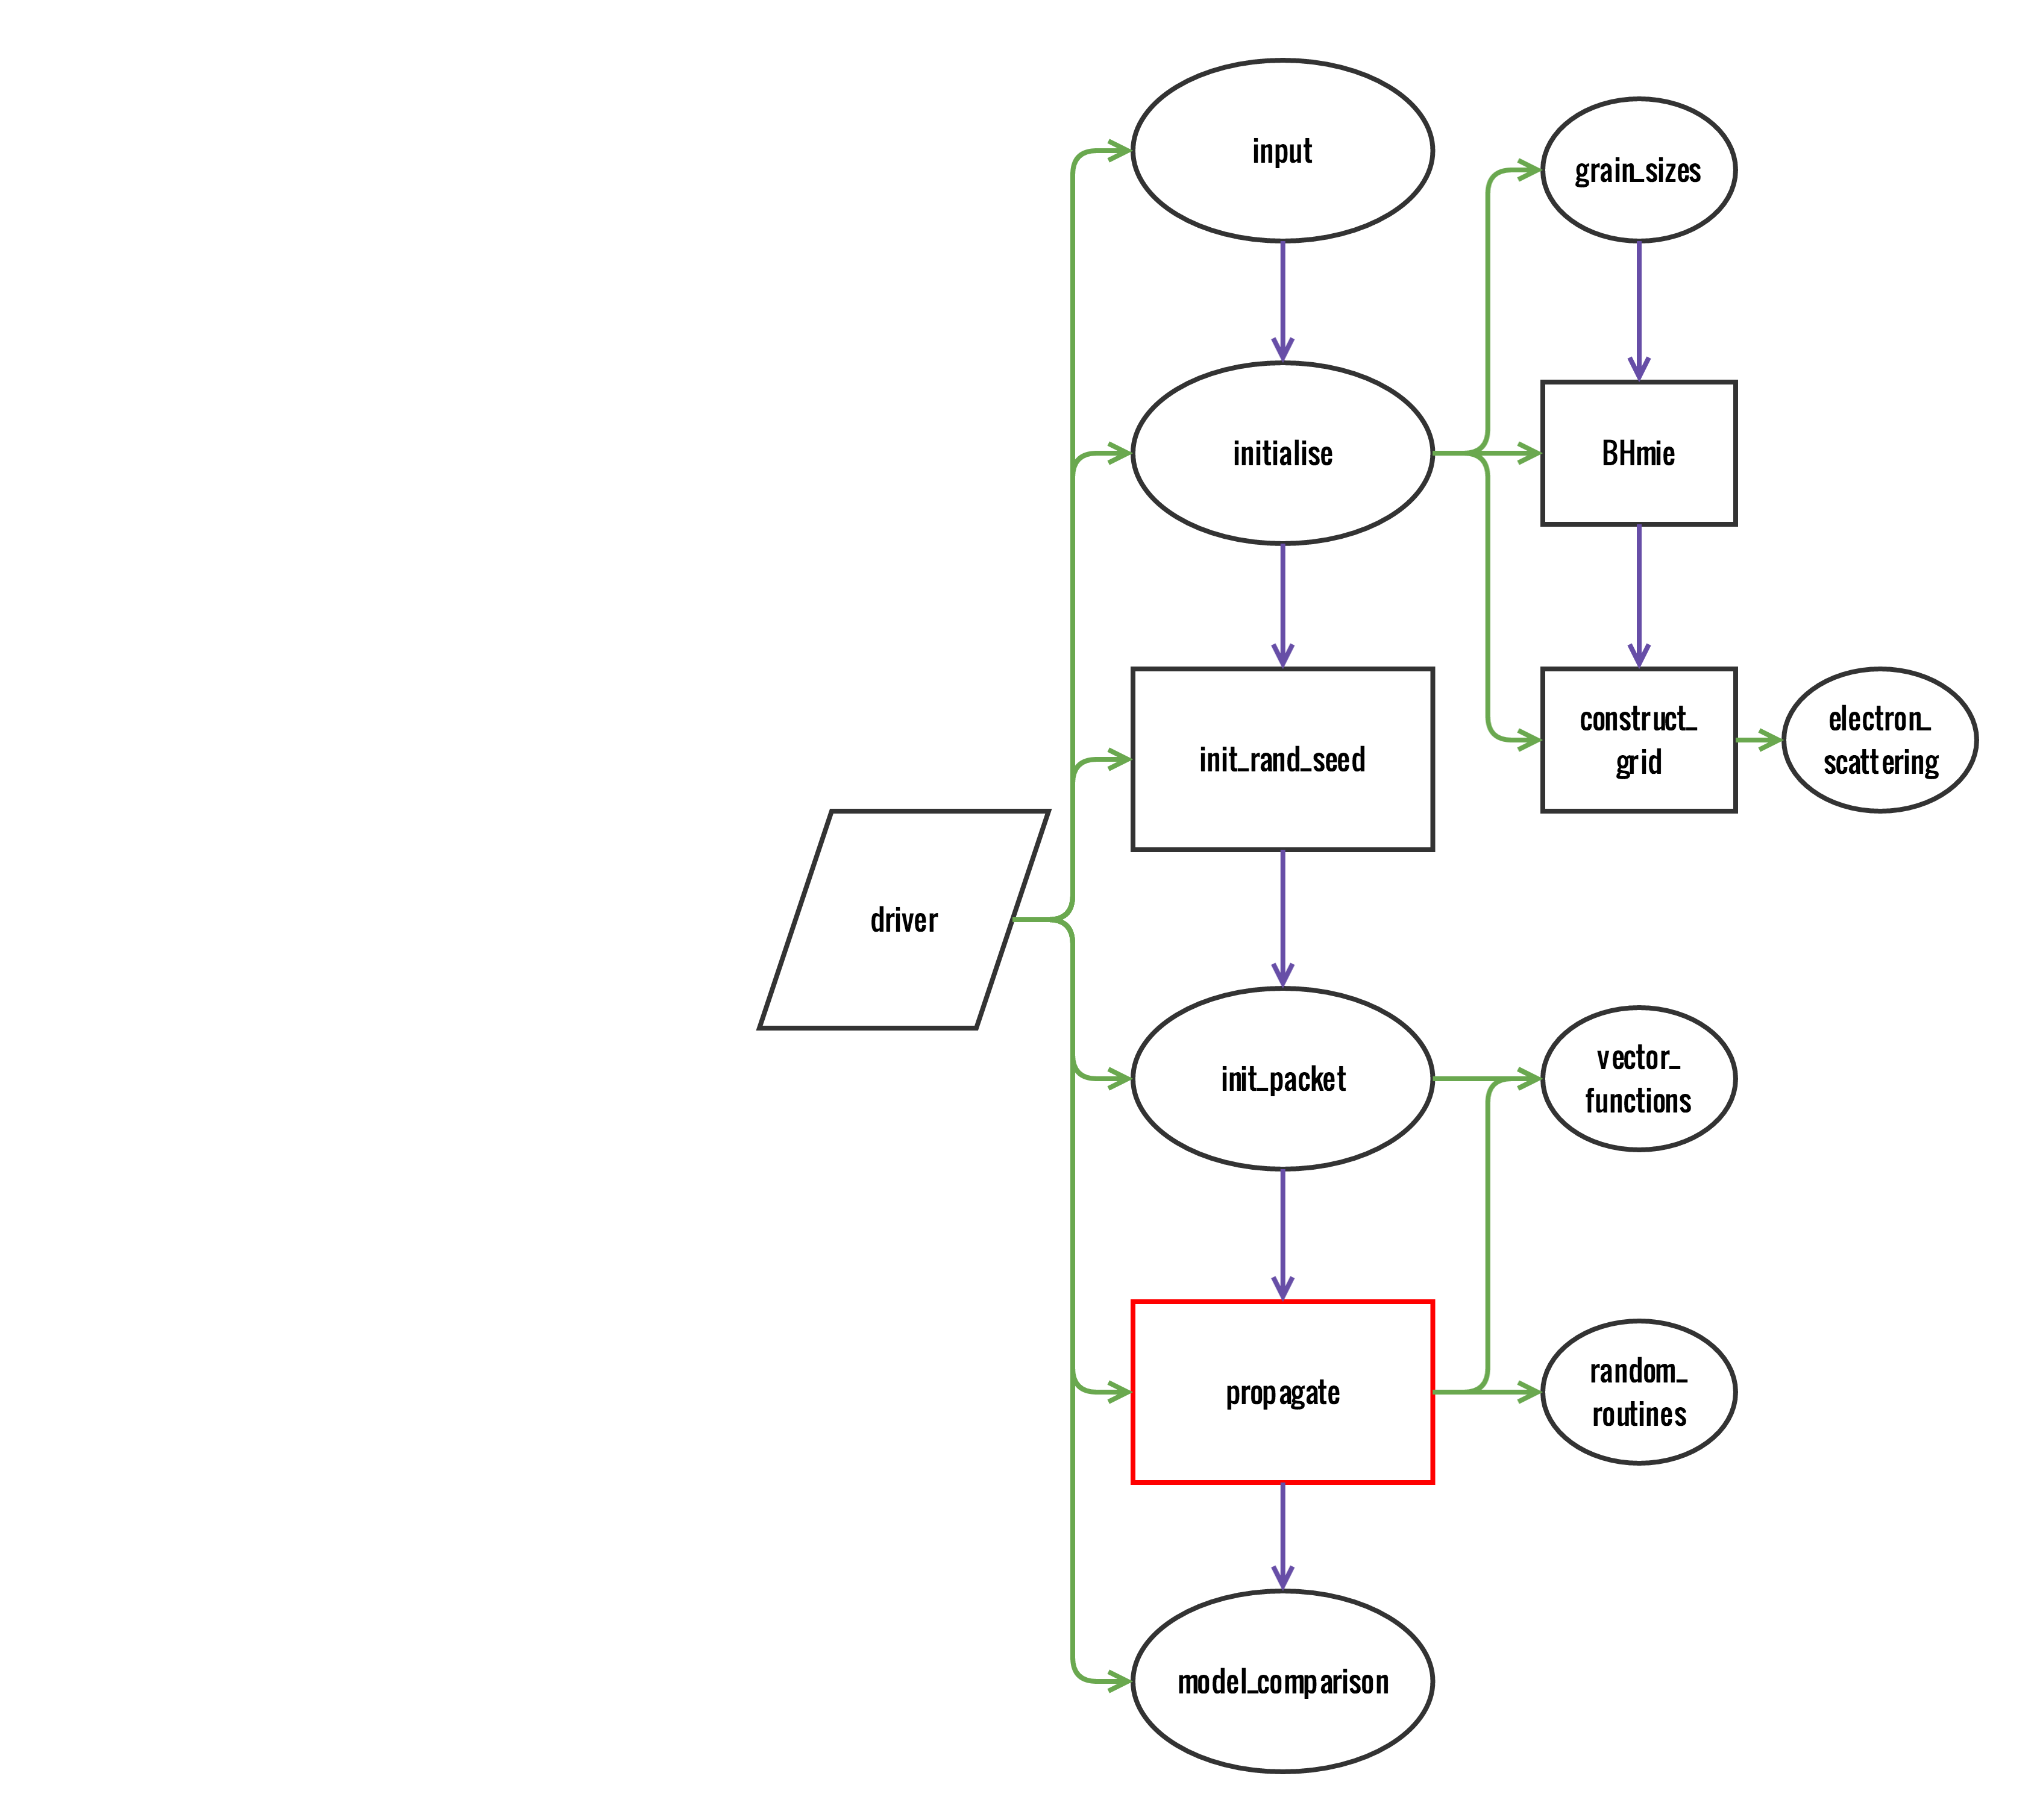
\includegraphics[scale=0.18, trim=430mm 20mm 30mm 25mm]{chapters/chapter2/code_modules_flowchart.png}
        \caption{A flowchart representing the hierarchy of modules and subroutines in the DAMOCLES code.  Ellipses represent modules and rectangles represent subroutines (the red rectangle is a recursive subroutine).  Green arrows indicate the dependence of a module or subroutine on previous modules or subroutines.  Purple arrows indicate the flow of the code.}
        \label{fig:flowchart_mods}
        \end{figure}

        
        \subsubsection{The input module}
        The \textit{input} module is where the primary input file is read into the code and all global variables are declared and assigned.  A number of logicals are assigned based on values declared in the input file and some simple calculations are performed that determine the inner and outer radii based on the maximum velocity specified and the epoch of consideration ($R_{out} = V_{max} \times t$).  A number of physical constants that are used throughout the code are also declared here as ``parameters", meaning that their value cannot be changed at any point in the simulation.
        
        \subsubsection{The initialisation module}
        The \textit{initialise} module acts as a driver to run all of the subroutines associated with initialising the program.  A number of dynamically allocatable arrays are declared allowing for a grid of densities to be calculated, a frequency grid to be stored and optical properties to be read in.  Arrays to store the emergent spectrum are also declared.  The calculation of dust opacities, which calls the \textit{grain\_sizes} subroutine and the \textit{BHmie} subroutine, is performed here.  For each species, the wavelength-dependent optical properties, $n$ and $k$, are read in and the Mie routine applied to every pair of frequencies and grain radii.  The resulting extinction and scattering efficiencies are summed over all grain radii for each wavelength, weighted appropriately, to calculate overall wavelength-dependent extinction and scattering opacities (see Section \ref{scn:grainsizes} for further detail).  These data are stored in an array that is accessed as necessary when packets are propagated through the grid.   
        
        The command to construct the grid is called before some basic statistics about the grid are calculated.  The average optical depth from $R_{in}$ to $R_{out}$ in both the V band and the rest-frame wavelength of the line being modelled are calculated and sent to stdout.  The average number density of grains in each cell is also computed and output.  Finally, the frequency array is constructed.
        
        This module is also where the `gridcell' derived type is declared.  A `gridcell' type was specified as it allowed for easy and clear access to any of a grid cell's properties as a packet passed through it.  The type consists of a number of arrays of real, integer and logical variables.  The properties recorded for each cell include the physical bounds of the cell in each axis, the mass and number dust densities,  the electron density, an identifying number (ID) and a logical clumped property. 
        
        \subsubsection{The grain size module}
        The \textit{grain\_sizes} module reads in the file that specifies the list of species to be used.  This file is a list of species detailing the name of the file containing the optical data for the species, the relative abundance of that species, the maximum and minimum grain radii and the exponent of the power law of the grain radius distribution.  It also declares how fine the grid of grain radii should be.  These properties are all read in by the \textit{grain\_sizes} module and a relative weight for each grain radius for each species is calculated here.
        
        The `species' derived type is declared in this module.  Similarly to the `gridcell' type, using a derived type allowed for the easy storing and accessing of a large number of properties of each species.  Many multi-dimensional arrays and scalars are stored for the `species' type including properties relating to the grain radius distribution, the density of a dust grain, the extinction and scatting opacities and the relative abundance of the species amongst others.  After the processing of the optical data for all species is completed, the calculated quantities are stored in arrays as components of the `species' type. 
        
        \subsubsection{The Mie approximation subroutine}
		The \textit{BHmie} subroutine is a standard routine that  was obtained from an online library of routines.  It is a modified version of the \citet{Bohren1983} Mie scattering routine.  The algorithm applies the mathematics described in Section \ref{needref} to determine the extinction and scattering efficiencies of a single size grain at a specified wavelength given its complex refractive index $n+ik$.
		
		\subsubsection{The grid construction subroutine}
		The \textit{construct\_grid} subroutine is called from within the initialisation module.  The purpose of this subroutine is to populate the grid, which is an array of derived type \textit{gridcell} and size $n_{cells}$ where $n_{cells}$ is the number of cells in the grid.   The bounds of the grid are initialised and the radii of all cells from the centre of the grid to the centre of the cell are calculated.  The density of each cell is then calculated according to a smooth power-law density distribution and scaled so that the total dust mass is equal to that specified in the input file.  If clumps are used then the total number of clumps is calculated and these are distributed throughout the grid stochastically according to the smooth density profile stipulated.
		This subroutine also calls the electron scattering subroutine contained within the \textit{electron\_scattering} module so that the electron density of a cell may be stored at the same point as the dust density.
		
		\subsubsection{The electron scattering module}
		The \textit{electron\_scattering} subroutine is a simple subroutine that is used to calculate the value of $K$ as described in equation \ref{eqn:es_distn}.  The total H$\alpha$ luminosity and the gas temperature are read in and the gas temperature used to determine the appropriate value of $q_{H\alpha}$ from Table \ref{tb:q}.  These values are then used to calculate the value of $K$ as described by equations \ref{eqn:kcalc1} and \ref{eqn:kcalc2}.  The variable is passed back to the \textit{grid construction} subroutine where it is used to calculate the electron density in each cell.  The electron densities will be used by the \textit{propagate} subroutine to calculate the electron scattering optical depth in each cell.
		
		\subsubsection{The random seed subroutine}
		The \textit{init\_rand\_seed} is a short subroutine that calculates a seed for the standard Fortran pseudo-random number generator (\textit{random\_number}).  It uses the system clock to generate the random seed and thus varies with every implementation of the code.  A seed is a number that is used as a ``starting point" for a pseudo-random number generator.  Varying the random seed ensures that a different set of random numbers is generated every time the code is run, which can be useful to ensure that any peculiar or interesting features of the outputted line profiles are definitely a product of the physical processes involved and not a result of random fluctuations in the simulation.  The more packets are used however, the more the Monte Carlo noise in the emergent line profile is reduced and the contribution from any anomalous packets should be insignificant.
		
		\subsubsection{The packet initialisation module}
		The \textit{init\_packet} module is responsible for the creation and emission of packets at the start of the simulation.  It is called from the driver for each packet.  By generating an array of five random numbers, the position and emission direction vectors in the rest frame of the emitter are calculated according to the formulae described in equations \ref{eqn:isotropic} to \ref{eqn:isotropic3}.  The scalar velocity of the emitter is calculated based on its radial position and this converted into a velocity vector by normalising the position vector and multiplying by the scalar velocity.  The velocity vector is passed to the Lorentz transforms subroutine contained in the \textit{vector\_functions}  module.  The frequency of the packet is also passed to this subroutine.  After the propagation direction vector and the frequency of the packet have been updated to the observer's rest frame, the grid cell in which the packet starts its path is identified and the code passes back to the driver to propagate the packet through the nebula.
		
		\subsubsection{The vector functions module}
		A number of vector functions are contained within the \textit{vector\_functions} module and are accessed throughout the program.  These include normalisation functions, conversions from spherical coordinates to cartesian and both forward and inverse Lorentz transforms.  It is the latter of these that are most important for the physics of the code.  The Lorentz functions are called for each packet at emission from the \textit{driver} and at every subsequent scattering event from within the \textit{propagate} routine.  As well as performing the necessary frequency shift based on the velocity of the scatterer or emitter, they also transform into and out of the rest frame of the particle thus ensuring that the packet is propagated through the nebula with a direction in the rest frame of the observer but that its new direction is sampled from an isotropic distribution in the rest frame of the emitting or scattering dust grain.  
		
		The $\beta$ and $\gamma$ values are calculated based on the input velocity vector.  The momentum 4-vector $\boldsymbol{P}$ is then multiplied by the Lorentz matrix $\boldsymbol{\Lambda}$ using the Fortran function \textit{matmul} to produce a  new frequency and a new direction vector in the appropriate frame of reference.  If a scattering event has occurred then the weight of the packet is also updated here.  The new direction vector, frequency and weight are then passed back to the propagate routine and the process repeated.   At each scattering event the inverse Lorentz matrix must first be applied to move from the observer's rest frame to the particle's.  A new direction vector must then be sampled from an isotropic distribution before applying the forward Lorentz transform to move back from the rest frame of the dust grain to the observer's frame.  The next step in the packet's trajectory may then be calculated in the \textit{propagate} subroutine.
		
		\subsubsection{The propagate subroutine}
		The \textit{propagate} subroutine is at the heart of the Monte Carlo simulation.  It is here that the trajectories of all packets in the simulation are determined.  The \textit{propagate} subroutine is a subprogram called a \textit{recursive subroutine}.  This allows the subroutine to call itself, at which point it will loop back to the start of the subroutine.  It will continue this process until a condition is reached that instructs it to return to the driver.  In this case a number of conditions will arrest the circulation of the packet. If the packet has escaped the outer radius of the ejecta or has been absorbed then the routine will pass this information along with the frequency and weight of the packet back to the driver.  The routine would also stop recurring if a packet has undergone a maximum number of scattering events (500 by default).  At this point it is deemed that the weight of the packet is so small as to be negligible and it is classified as ``inactive".  This prevents the code from lagging by becoming stuck on a particular packet that has become trapped in a region of high density and albedo. It is noted that if this is the case for a large number of packets then a bias may be introduced - packets emitted in particularly high density regions may be discarded more frequently than those emitted in less dense regions.  The number of packets that are deemed ``inactive" is output as a percentage of the total number of packets employed at the start of the simulation as a check for the user.  In practice, unless the albedo of the dusty medium is extremely high and the medium is very dense, this is rarely an issue (for an average simulation with $10^7$ packets, normally only one or two are discarded for this reason). 
				
		\begin{centering}
		\begin{figure}
		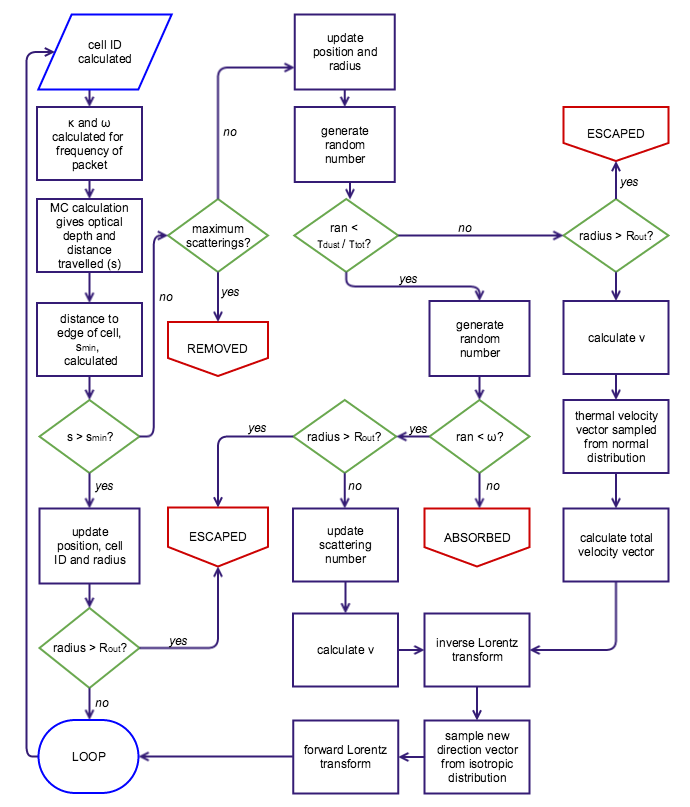
\includegraphics[scale=0.165, trim=1180mm -20mm 28mm -20mm]{chapters/chapter2/propagate_module.png}
		\caption[A flowchart representing the processes that occur in the \textit{propagate} subroutine]{A flowchart representing the processes that occur in the \textit{propagate} subroutine.  The life of a packet passing through the grid may be determined by following the flowchart starting at the blue parallelogram (top left).  Purple oblongs indicate a standard step in the evolution, green diamonds indicate that a determination must be made, red boxes mean that the packet's evolution has concluded as it has escaped, been absorbed or been removed and the blue rounded oblong indicates a return to the start of the routine.}
		\label{fig:flowchart_propagate}
		\end{figure}
		\end{centering}
		
		There are a number of processes that take place in this module in order to propagate a packet through the nebula accurately.  A full pictorial representation of the procedures that are implemented in this module may be found in the flowchart in Figure \ref{fig:flowchart_propagate}. For each packet in each grid cell, the optical depth in that cell is calculated based on the dust density and the opacity at the wavelength of the current packet.  These are obtained by interpolating between discrete opacities at points in the frequency array.  At this stage, the Monte Carlo technique is applied in order to determine the distance travelled by the packet by sampling from the cumulative probability distribution.  This displacement is then compared to the distance from the packet's current location to the edges of the grid cell in order to ascertain whether or not the packet escapes the cell.  If it does escape then the packet advances to the bounds of the current grid cell and the process is repeated in the next cell.  If it does not escape then an event occurs.  In this case, random numbers are sampled in order to determine whether the packet experiences electron scattering, dust scattering or absorption.  If the packet is absorbed then it is removed from the simulation, the \textit{propagate} subroutine is arrested and the code returns to the driver to emit a new packet.  If it is scattered then the velocity vector is calculated.  In the case of electron scattering this involves considering the thermal velocity component as well as the bulk velocity at that radius.  The Lorentz transforms are applied based on the velocity vector and the frequency and weight of the packet are updated.  A new direction of propagation is sampled in the scatterer's rest frame from an isotropic distribution and is transformed into the observer's rest frame.  The routine is recalled to start afresh with the new propagation direction. 
		
		\subsubsection{The random routines module}
		The \textit{random\_routines} module contains a single subroutine which is, like the \textit{BHmie} routine, a standard routine obtained from an online library.  It allows for a random velocity vector to be sampled from a normal distribution with specified mean and standard deviation.  The standard deviation is calculated as per equation \ref{eqn:sigma_maxwell} and passed to the subroutine which samples a random 3-dimensional vector from the normal distribution with the specified standard distribution and zero mean.  This is passed back to the \textit{propagate} routine where it is added to the bulk velocity in order to determine the overall velocity of the scattering electron.
		
		\subsubsection{The model comparison module}
		The \textit{model\_comparison} module is responsible for post-processing the outputted line profile and comparing the model results with inputted observed data.  The routine interpolates between two model frequency points to obtain a flux value at each frequency point of the observed line profile.  Both profiles are then normalised such that the total flux is unity.  A MSE calculation is then performed as per equation \ref{eqn:chi2}. The smaller the value of MSE, the better the fit is.  It should be noted however that data with a poor signal-to-noise ratio will have an inherently large MSE than data with a good signal-to-noise ratio.
		
		
		\subsection{OpenMP Parallelisation}	
		\label{scn:open_mp}
		
	Monte Carlo simulations are exceptionally well-suited to parallelisation.  The path of each packet through the nebula is unaffected by the transport of any other packet.  It is therefore possible to run multiple instances of the \textit{propagate} module at once by using several threads.  Since the vast majority of the processing power of the simulation is driven from this module, it is theoretically possible to achieve a nearly linear speed-up; i.e. if the number of cores is doubled, the run time should be approximately halved.  %check for threads, cores or processors? 
	
	DAMOCLES was parallelised using OpenMP.  OpenMP is an Application Program Interface (API) that allows for shared-memory parallel programming in Fortran and C/C++.  OpenMP causes the code to be run serially on a single processor until a parallel region is reached.  At this point the single master thread branches into multiple threads, and multiple instances of the same section of code are run on each.  In DAMOCLES, this splitting occurs at the start of the loop which controls the emission and propagation of packets from each shell.  If, for example, $10^7$ packets are emitted and 5 threads are used, then approximately $2 \times 10^6$ packets will be independently processed on each thread.  Practically however, the OpenMP keyword \textit{dynamic} is declared ensuring that, as soon as each thread has finished processing a packet, it immediately moves onto the next one.  If the \textit{static} keyword were specified instead then the number of packets to be processed would be equally divided between the threads at the start of the loop.  In this case, if, by random chance, one thread happened to have significantly more absorbed packets than another, then potentially utilisable processing power would be lost as the core waited for the others to finish.
	
	At the start of the parallel region variables accessed within the shared region are specified as shared or private.  Private variables are not seen by other threads and allow the value of a single named variable, for example ``frequency", to have different values on different threads.  Shared variables have the same value regardless of the thread number, for example, ``grid cell density".  As each packet escapes, its weighted energy must be added to the final energy array.  It is important that two threads do not attempt to alter the value of this shared array at the same time as data may be lost or corrupted. This section of code is therefore enclosed inside a \textit{critical} region.  This instruction ensures that code in this block is to be executed by only one thread at a time.  Extensive testing was performed to ensure that outcomes were not affected by the implementation of a parallel environment.
	
	For further information about the OpenMP API please refer to \textit{https://www.openmp.org}.
	
	\subsection{Input}
	
	There are a significant number of parameters that may be varied in the code.  Many of these are important variable parameters that will be the parameters of interest when modelling.  However, there are also a significant number of variables that allow other properties of the model to be controlled.  All parameters can, broadly,  be divided into one of three categories:  properties of the emitted rest-frame line or doublet, properties of the dust and gas in the ejecta and properties of the grid and code architecture.  I list all the variables that are input in the primary input file in Table \ref{tbl:input} and will here briefly describe the basic meaning and function of each one.
	
	\begin{table}[htdp]
	\caption{The input variables read in from the input file and example values}
	\begin{center}
	\def\arraystretch{1.5}
	\begin{tabular}{l r c c l r}
	\toprule
	Input Variable & Example Value &&& Input Variable & Example Value\\
	\midrule
	lambda1\_0 & 636.3 &&& MD\_tot & 1.0e-4\\
	L\_tot & 0.003 &&& l & 1.0\\
	L\_Halpha & 0.005 &&& q & 1.3\\
	doublet & 1 &&& b & 2.0\\
	lambda2\_0 & 630.0 &&& gas\_shell & 1\\
	L\_ratio & 3.1&&& v\_max\_gas & 8000\\
	ES & 1 &&& Rrat\_gas & 0.05\\
	ES\_temp & 10000 &&& l\_gas & 1.0\\
	LS & 0 &&& q\_gas & 1.5\\
	VelShift & 1 &&& b\_gas & 2.0\\
	MF & 0.5 &&& ncells & 50\\
	FF & 0.1 &&& n\_packets & 1e8\\
	dayno & 680 &&& n\_bins & 1000\\
	v\_max & 5000 &&& n\_shells & 100\\
	Rrat & 0.2 &&& dustfile & ``species\_file.in"\\
	\bottomrule
	\end{tabular}
	\end{center}
	\label{tbl:input}
\end{table}%

\vspace{0.8cm}

\subsubsubsection{Properties of the emitted rest-frame line or doublet}
\subsubsubsection{lambda1\_0 }  

This is a real number that specifies the initial rest-frame monochromatic wavelength at which packets are emitted in nanometres.  If a doublet is to be modelled then this represents the wavelength of one of the singlets.

\subsubsubsection{L\_tot }

L\_tot is the total luminosity of the line in units of $10^{40}$ ergs s$^{-1}$.  The initial energy of each packet ($E_0$) is therefore L\_tot divided by the total number of packets used in the simulation (n\_packets). For lines which have calibrated observed fluxes, this allows the flux of the line to be modelled in addition to the normalised shape.  This variable is also used to estimate the undepleted luminosity of the observed line when it is initially emitted from the ejecta.

\subsubsubsection{L\_Halpha}

Similar to L\_tot, L\_Halpha is the total luminosity of the H${\alpha}$ line.  In the case of H${\alpha}$ modelling, this value should be the same at the value of L\_tot.  This variable is used in the calculation of the electron density and it is not necessary to specify it unless the electron scattering environment is switched on (see section \ref{scn:ES} for further details).  

\subsubsubsection{doublet}

This is an integer of value 1 or 0 that indicates the use or otherwise of the doublet environment.  If set to 1 it triggers the doublet logical in the code to be initialised to \textit{true}.  The code will then read in the values of {lambda2\_0} and {L\_ratio} in order to initialise packets with two different starting monochromatic wavelengths.  Packets are processed through the nebula as normal before being collated in bins weighted according to both their history and the intrinsic flux ratio of their parent singlet.

\subsubsubsection{lambda2\_0}

This is a real number that specifies the initial rest-frame monochromatic wavelength of packets emitted from the second singlet in a doublet environment.  The wavelength is specified in nanometres.

\subsubsubsection{L\_ratio}

This real number gives the ratio between the respective luminosities of singlets in a doublet environment.  The ratio should be declared as the flux at lambda1\_0 divided by the flux at lambda2\_0.  It is expected that the doublet environment will generally be used to model forbidden lines, especially the [OI]$\lambda$6300,6363\AA\ doublet, where the intrinsic flux ratio between the singlets may be theoretically determined.

\vspace{0.8cm}

\subsubsubsection{Properties of the dust and gas in the ejecta}
\subsubsubsection{ES}

This keyword is similar to the doublet keyword in that, by setting it equal to 1 or 0, it indicates the use or otherwise of the electron scattering environment.  If it is set to 1 then it initialises the electron scattering logical in the code to \textit{true}.  If the electron scattering environment is switched on then this triggers the calculation of electron densities for every cell in the grid.  This density contributes to the total optical depth of a cell and, as packets are propagated through each cell, they will experience an electron scattering event with probability $1-e^{\tau_e}$, where $\tau_e$ is the electron scattering optical depth.

\subsubsubsection{ES\_temp}

 When the electron scattering environment is switched on, it is necessary to calculate the electron density of each cell in the grid.  In order to do this an average gas temperature must be specified to allow for $q_{H\alpha}$ to be determined.  DAMOCLES will not accept any value for this input variable; only 5,000K, 10,000K and 20,000K will be accepted.  These are thought to be a representative range of temperatures for the ejecta of supernovae at epochs where electron scattering still has the potential to influence observed line profiles.  These specific values were selected since they are the values of $q_{H\alpha}$ that are given in \citet{Osterbrock2006}.

 \subsubsubsection{MF}

 If this keyword (short for mass fraction) is set to 0 then a smooth density distribution of both gas and dust will be constructed.   If it is not however, then this will automatically initialise the clumping logical present in the code to \textit{true}.  The value specified should be between 0 and 1 and gives the total fraction of the dust mass that should be located in clumps.  The remaining fraction will be smoothly distributed according to the power-law density profiles declared in the input file.

 \subsubsubsection{FF}

 If the clumping environment is switched on (using the \textbf{MF} keyword) then \textbf{FF} declares the total filling factor of the clumps.  The filling factor is defined as the fraction of the total volume of the ejecta that is occupied by clumps.  For a fixed clump size, this parameter effectively determines the number of clumps to be used.  Once the number of clumps to be used has been determined, the mass fraction then determines the density of the clumps.
 
 \subsubsubsection{dayno}

 This keyword represents the epoch being modelled.  In combination with the declared maximum velocity, it is used to consistently calculate an outer radius as 
 \begin{equation}
 R_{out}=8.64 \times 10^{-6} \Big( \frac{t}{\mathrm{days}} \Big) \Big( \frac{v_{max}}{\mathrm{kms^{-1}}} \Big)
 \label{eqn:Rout_calcn}
 \end{equation}

 \noindent where $R_{out}$ is in units of $10^{15}$cm.

 \subsubsubsection{v\_max}

 This is the maximum velocity used in the code.  It is assumed to be the velocity at the outer radius of the ejecta and is used to construct a velocity profile of the form
 \begin{equation}
 v(r) = v_{max} \Big( \frac{r}{R_{out}} \Big)^l
 \label{eqn:vel_law}
 \end{equation}

 where $l$ is also declared in the input file and $R_{out}$ is calculated based on the epoch and the maximum velocity.

 \subsubsubsection{Rrat}

 This number is the ratio between the inner and outer radii.  Once the outer radius has been calculated as per Equation \ref{eqn:Rout_calcn}, this ratio is used to calculate the value of the inner radius.

 \subsubsubsection{MD\_tot }

 This real number specifies the total dust mass to be distributed throughout the grid in solar masses ($M_{\odot}$).

 \subsubsubsection{l}

 $l$ is the exponent of the radial velocity law in the code as per equation \ref{eqn:vel_law}.

 \subsubsubsection{q}

 $q$ describes the relationship between the radial dust density distribution and the emissivity distribution.  It is the exponent of the emissivity distribution as a function of density such that $i(\rho) \propto \rho^q$ where $i(\rho)$ is the emissivity at a given density.  Though this parameter may take any real value, it is frequently fixed to be $i(\rho) \propto \rho^2$, i.e. proportional to the product of the recombining proton and electron densities in the case of H$\alpha$ and to the product of the neutral oxygen and electron densities in the case of collisionally excited [O~{\sc i}] emission.


 \subsubsubsection{b}

 This parameter describes the value of the exponent of the dust density distribution in terms of radius such that $\rho \propto r^{-b}$.

 \subsubsubsection{gas\_shell}

 This flag may be set to 0 or 1 to indicate that dust and gas are coupled or decoupled respectively.  If it is set to 1 then the ``decoupled" logical in the code is set to \textit{true} and the gas follows a density distribution that is independent of the density distribution followed by the dust.  The following five parameters specify the geometry of the emitting gas.  It is worth noting that in the case where gas and dust are coupled to each other, the gas follows the same distributions as specified for dust by the parameters described above. 

 \subsubsubsection{v\_max\_gas}

 This is the gas analogue of the v\_max parameter described above.  

 \subsubsubsection{Rrat\_gas}

 This is the gas analogue of the Rrat parameter described above.  

 \subsubsubsection{l\_gas}

 This is the gas analogue of the parameter $l$ described above.  

 \subsubsubsection{q\_gas}

 This is the gas analogue of the parameter $q$ described above.  

 \subsubsubsection{b\_gas}

 This is the gas analogue of the parameter $b$ described above.  

\vspace{0.8cm}

 \subsubsubsection{Properties of the grid and code architecture}
 \subsubsubsection{LS}

 For an initially symmetric distribution of gas and dust, it is not necessary to specify a line of sight as all lines of sight will produce the same profile.  It is therefore more efficient to collect all packets that escape regardless of their direction of flight.  However, if an alternative, axisymmetrical or asymmetrical geometry is adopted then the ability to specify a line of sight is important.  If this keyword is set to 1 then the ``line of sight" logical will be initialised as \textit{true}.  Only packets that escape within a cone of vertical angle $\pi/6$ will be collected.  Clearly, in practice, the angle would be very much smaller but it is prohibitively expensive to run enough packets through the simulation that enough are collected to achieve a reasonable resolution when a very small vertical angle is adopted.  A representation of this construction is presented in Figure \ref{fig:LOS}.

 \begin{centering}
 \begin{figure}
 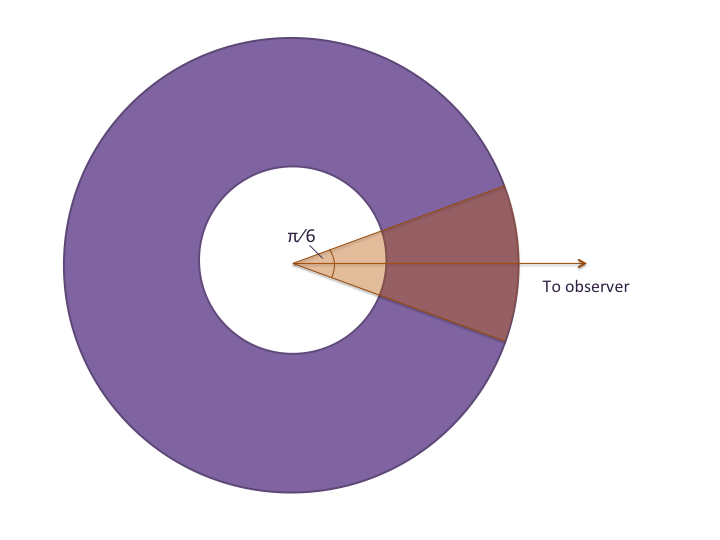
\includegraphics[scale=0.55, trim=-25mm 10mm 29mm 0mm]{chapters/chapter2/LoS_diagram.png}
 \caption{Schematic representing which packets are collected when the line of sight environment is switched on.  Packets that contribute to the emergent line profile are those that escape the nebula within a cone with vertical angle $\pi/6$.}
 \end{figure}
 \end{centering}

 \subsubsubsection{VelShift}

 This is another environment flag.  As a packet is transported through the nebula it may experience repeated scattering events that shift its original frequency beyond that expected from the maximum theoretical velocity.  It is discused in depth in the next chapter how this process of ``velocity shifting" may result in a profile that exhibits an extended red wing.  It is useful for the purposes of comparison and investigation to be able to turn off this process of repeated scattering events so that the only frequency shift experienced by a packet is at emission.



 \subsubsubsection{ncells}

 Each axis is split into this number of divisions.  The total number of cells in the grid is therefore ncells$^3$.


 \subsubsubsection{n\_packets}

 This variable determines the number of packets to be emitted and processed through the grid.  This parameter is particularly important for achieving a resolution that is high enough to give representative results.  The larger the number of packets used, the less noise is present in the final profile.  The Monte Carlo process introduces noise that can sometimes be construed as a result when it is in fact a numerical artefact.  Using a large number of packets reduces this risk and improves the output of the model.  In general, the more dense an environment, the more packets it is necessary to use.  This is because any packets which are absorbed are removed from the simulation and therefore reduce the desired resolution.  Since the vast majority of the total processing power is used to propagate packets through the grid, an increase in the number of packets results in a significant decrease in runtime. Optically thick simulations of dust with a very high or a very low albedo have a significantly longer runtime than optically thin scenarios.  When choosing this parameter, a careful balance must be found between the total runtime and the desired resolution. 


 \subsubsubsection{n\_bins}

 This value gives the total number of divisions in the frequency array and thus determines the overall frequency resolution of the outputted line profile.  Since the resulting profile is in fact a histogram binned into a frequency array, it is important that these divisions are fine enough to provide a seemingly continuous line profile.  Apparent jumps or discontinuities could be produced if too few bins are used.

 \subsubsubsection{n\_shells}

 This parameter controls the total number of shells the ejecta is divided into at the start.  If a particularly steep radial profile is adopted for either the velocity profile or the density profile then the user may wish to increase the number of shells used to compensate.  Increasing the number of shells will have an effect on the overall runtime, but this will be insignificant in comparison to altering the number of packets.  

 \subsubsubsection{dustfile}

 Finally, this string gives the name of the input file that itemises the list of species, their relative abundances and size distributions.

 \begin{table}
 \caption{List of all outputs and example values produced by the DAMOCLES code.}
 \begin{center}
 \def\arraystretch{1.5}
 \begin{tabular}{ l  r}
 \toprule
 Output & Example Value \\
 \midrule
 Total number of cells      & 125000 \\
 Number of grid cells inside ejecta   & 65544 \\
 Total volume of supernova (10$^{42}$ cm$^3$)   & 304523264 \\
 Volume of a grid cell / Volume of a clump (10$^{42}$ cm$^3$)   & 4668.52\\
 Width of a grid cell (cm) &   1.67e+15\\
 \midrule
 Mass check (calculated as $\rho V$)   & 6.03e-04 \\
 \midrule
 Average grain number density (cm$^{-3}$)  & 1.96e-09\\
 Extinction to rest-frame wavelength  & 2.94e-08 \\
 Scattering extinction to rest-frame wavelength  & 1.63e-08 \\
 Albedo for rest-frame wavelength & 0.554 \\
 Average optical depth to rest-frame wavelength  & 2.062 \\
 Average optical depth in V band  & 2.18 \\
 \midrule
 Average electron density (cm$^{-3}$) & 71509.1 \\
 Average electron scattering optical depth &   1.31e-02\\
 \midrule
 Total number of packets      &          100000\\
 Number of active (propagated) packets      &          100000\\
 Number of inactive packets        &            0\\
 Number of absorbed packets      &          82949   \\
 Percentage of absorbed packets out of all active packets & 82.95 \\
 Number of packets in line of sight  & 17050       \\
 Percentage of escaped packets in line of sight & 100.0 \\
 \midrule
 Estimated undepleted luminosity ($10^{40}$ ergs s$^{-1}$)  & 1.10e-05\\
 Total (depleted) luminosity ($10^{40}$ ergs s$^{-1}$) & 1.90e-06\\
 Total energy absorbed ($10^{40}$ ergs s$^{-1}$) &  1.57e-06\\
 Energy per active packet ($10^{40}$ ergs s$^{-1}$) & 1.90e-11\\
 \midrule
 MSE	& 0.3557  \\
 \bottomrule
 \end{tabular}
 \end{center}
 \label{tb:outputs}
\end{table}%

\subsection{Output, Post-Processing and Visualisation}

The primary output file contains details of the emergent line profile.  Three columns are written out to the file at the end of the simulation.  These are the wavelength, velocity and flux of the modelled line profile.  Another output file is also produced by the \textit{model\_comparison} module.  This file prints both the inputted observed line profile and the outputted emergent line profile to one file in the same velocity bins.  This allows for easy plotting.  The columns printed in  this file are wavelength, modelled flux and observed flux. The total flux is normalised to unity for both line profiles.  Both of these files may be represented graphically in a straightforward fashion using any plotting package.  In addition to these output files, a number of useful quantities are also calculated by DAMOCLES and output to \textit{stdout} throughout the course of the simulation.  If desired, the user may direct the \textit{stdout} to a file for a record of these quantities.  A list of all quantities output by DAMOCLES is given in Table \ref{tb:outputs}.

Throughout my modelling, I use standard and custom routines written with MATLAB to plot line profiles, both modelled and observed.  I also use MATLAB to process some of the data.  For example, where I have observations with accurate observed fluxes, I scale the modelled profile to the observed profile so that fluxes remain to scale.  This is initially performed by a custom MATLAB routine which smooths the modelled data to reduce any Monte Carlo noise before identifying the maximum flux value.  Identifying the peak flux of the observed line profile allows the modelled profile to be automatically scaled.  Any inaccuracies in the scaling may then be easily adjusted manually.  I also use MATLAB for any other illustrative graphs or plots, for example, the plots in Figure \ref{fig:grid} were generated in MATLAB using its 3D-scatter plotting function.

\section{Further Developments}
\label{limitations}

The modular structure of DAMOCLES allows for easy implementation of additional functionality in the future.  By simply adding extra modules, extra physics can be included in the code.  There is potential for this code to be expanded in a number of directions.  An immediately apparent development involves the dust itself.  Treatment and understanding of the dust in the ejecta is crucial to understanding the shape of the line profile.  The ability to place different species in different locations within the ejecta is not currently included.  This would allow for stratified or asymmetrical distributions of dust species motivated by the potentially discrete locations of the parent elements.  Similarly, streamlining the ability to model arbitrary density distributions and geometries would allow for more complex and accurate modelling of supernova ejecta.  The ejecta of SN~1987A, for example, is known to have an asymmetric distribution which could potentially affect the contour of the line profile.

As mentioned previously, dust grains are rarely perfectly spherical and can be far more complicated in shape.  It might be of interest to include a module that treats a continuous distribution of ellipsoids as mentioned in Section \ref{needref} in order to more accurately model the effects of dust grains.

More widely, supernova explosions can sometimes result in radiation that is polarised.  By including the capacity to model polarised radiation in the code, we may able to glean further information about the distribution and nature of dust forming within the ejecta.  It would also be theoretically possible to expand the code to become a fully self-consistent radiative transfer code or to include certain approximations (e.g. the Sobolev approximation) to allow for full spectral modelling throughout the optical and infrared.

Aside from the development of the code directly, the current process of manual fitting can be laborious and has the potential miss potentially good fits due to the large number of variable parameters.  I have completed some work over the course of this PhD wrapping DAMOCLES in a MCMC (nested sampling) routine that allows for a more thorough investigation of parameter space resulting in a full multivariate probability distribution.  For reasons of time, the research presented in the following chapters was performed using manual fitting but further work finishing the implementation of this routine or a similar one would be invaluable in the future.





